\chapter{Asynchronous Editing Algorithm}
\label{chap:algorithm}

The way the concepts presented in the previous chapters were put to work together in order
to develop our novel asynchronous text editing system is described in this chapter. We
start by presenting the structure of the text document we work with and mention how it
enables us to achieve better performance, both in terms of algorithm efficiency and bandwidth
consumption. Then we carry on by discussing the operation types that exist in our system and
also present our implementation of basic and advanced operation transformations. The most
important part of this chapter focuses on the description of the three stages of the
copy-modify-merge asynchronous system (the commit, the update and the checkout stage).
In the end we cover some additional facilities our system offers and several performance
considerations.

\section{Tree representation of the text document}

The vast majority of collaborative text editing systems that exist nowadays start with
the assumption that a text document is represented as a sequence of characters and
simply take it from there. None of the research work we have studied (concerning
asynchronous collaborative text editing systems) even mentioned
the possibility of using any representation other than the classical one, let alone
think about the advantages that could be drawn from an alternative representation.
Using a linear view of the document usually implies that the only operations the system
ever works with are insertion and deletion of characters. Even though there are variants
of systems which allow the insertion and deletion of more than one character with a
single insert/delete operation, still the essence is that the document is viewed as
a series of characters with no additional structure. This brings several serious
disadvantages to the system as a whole, disadvantages which we shall try to outline below.

All algorithms (regardless of how they work) relying on operation transformation keep
a log of already executed operations in order to compute the proper execution form of
new operations. In systems using a linear representation of the document all past
operations are stored into a single common buffer (the per document buffer). When a
new set of operations (performed by some other user) from the repository has to be
merged into the local document, all operations from the set have to be compared to every
single operation from the local log, regardless of the fact that they might be referring
to completely different logical sections of the document. There is simply no way to
avoid this when linear representations are used. A great loss of efficiency arises
from this since the numbers used to compute the running time of the algorithms tend
to be much higher (i.e. the $n$ that appears in the efficiency formula
of the algorithm, the $O(f(n))$ would be significantly higher - directly proportional
to the length of the editing session - when all operations have to be
compared one to another as opposed to when massive operation separation can be employed;
it is enough to think of $O(n^2)$ algorithms in order to realize the improvements in running
time that can be obtained if operations can be separated in very many smaller groups
and compared separately). This is evermore worse when we realize that,
statistically speaking, most of the time users working together on a document work
on totally different parts of it. It is very seldom that two users actually work
on the same section of a document. This means that not only would we have a theoretical
efficiency improvement, but we would have an improvement which would appear very
often in practice.

Aside from the running time of algorithms, we can also sketch another disadvantage of
linear representation, namely the increased bandwidth usage.
In order to understand this, think of the two following ways of expressing the creation
of the sentence \emph{``We dance and the music dies''}. The way a linear system does
this is by generating a separate operation for the insertion of each character, something
like [Insert(0,'W'), Insert(1,'e'), Insert(3,'\verb*+ +'), Insert(4,'d'), \ldots].
On the other hand, a system using a more sophisticated way of representing documents
could simply achieve this with one operation only: [InsertSentence(0,'We dance and the
music dies')]. Even though the characters themselves occupy the same amount of space,
the overhead (position parameter, for example) of the second way of representation
is infinitely smaller than that of the first way. And this is just one sentence we
are talking about. Extrapolate this to the case of a full-fledged document and you
will easily understand why the use of bandwidth capacity is way more efficient when using
a tree representation.

The final issue we would like to mention is that of granularity level. When working with
linear representations, the user is constrained to one single level of granularity, namely
that of character granularity. The impact of this is that, even though syntactic consistency
is ensured, there is simply nothing that can be done in what semantic consistency is concerned. To
understand this, think of two users working with the sentence ``We danc and the music
dies'' (notice the missing 'e' from the word 'dance'). Say the first user adds an 'e'
at the end of 'danc' in order to obtain ``We danc\textcolor{red}{e} and the music dies''.
The second user, noticing the problem as well, decides to solve it by changing 'danc'
to 'wait', thus transforming the sentence to ``We \textcolor{blue}{wait} and the music dies''. A traditional
system based on linear representation of documents will at best be able to merge the
two changes in order to obtain ``We \textcolor{blue}{wait}\textcolor{red}{e} and the music dies'', which
is obviously not what any of the users wanted. This is because there is no way for
the users to specify what the basic semantic unit they want to be working with should be. If, for instance, it
would be possible to say that changes made to the same word are \emph{always} conflicting
(i.e. work at the word granularity level instead of the character granularity level)
the problem above would be solved. However, the exact same situation could happen
when using word granularity level if two users insert two different words in a sentence
in order to correct it (each of which, taken separately, rendering the sentence correct),
but the system puts both words in the sentence, generating a nonsense sentence
all over again (since the two words put together make no sense). Why not work at the
sentence granularity level then (i.e. two operations making changes to the same sentence
are \emph{always} conflicting)? The idea is that different granularity levels are appropriate
for different projects and it should be the user who decides what semantic unit (s)he
should be using. However, linear representation systems do and can not offer this option
to the user because they are unaware of document structure.

Given all these disadvantages, it is clear that there are lot of immediate improvements
one can think about. And this is exactly what we have done. We thought of improvements.
In order to address the issues mentioned above, the first (and most important) step
was to design a way of representing the text document structure which would then allow
the use of improved algorithms. The remaining of this section will describe this structure.

The model we propose (based on the one developed in our group and described in \cite{ignat02}
and \cite{ignat03}) is a hierarchical one which views the document as a collection
of paragraphs, the paragraph as a collection of sentences, the sentence as a collection
of words and the words as a collection of characters. Each of this represents a different
level of granularity the user can work at. These levels correspond to common semantic
elements used in the natural language. Even though our current implementation works with
a fixed height tree, the employed algorithms were designed and written in such a way that
the actual significance of the level is not taken into consideration, such that they
can be applied in their current form on virtually any other kind of tree representation
of a document (regardless of the height of the tree). For instance, in the case of writing
a book, the hierarchical structure of the document would consist of the following units
of granularity: book, chapter, section, paragraph, etc. However, in what follows we
are going to focus only on the text documents corresponding to the levels of abstraction
presented above. We assigned each of the abstraction units a different numeric level:

\begin{itemize}
\item document level = 0
\item paragraph level = 1
\item sentence level = 2
\item word level = 3
\item character level = 4
\end{itemize}

\emph{Note: given that the numbers increase as we go down in the tree, let us mention,
for the sake of clarity, that whenever we say lower/higher level of the tree, we see
the document level as the highest level and the character level as the lowest level.}

The best way of rigorously defining what our document tree means is to start with
the formal definition of the generic node of our tree:

\begin{defi}
A \emph{node} is a structure of the form $N=\{level,length,content,children,log\}$, where

\begin{itemize}

\item \emph{level} represents the level in the tree of the node; $level \in \{0,1,2,3,4\}$.

\item \emph{length} represents the length of the node,

$\qquad length=\left\{
\begin{array}{ll}
1 & \text {, if }level=4; \\ 
\sum\limits_{i=1}^{n}length(child_{i}) & \text{, otherwise.}
\end{array}
\right.$

$f(x)=\left\{
\begin{array}{ll}
x-1, & x < 10 \\
x+1, & x \ge 10
\end{array}
\right.$

\item \emph{content} represents the content of the node, defined only for leaf nodes

$\qquad content=\left\{
\begin{array}{ll}
\text{undefined} & \text{, if }level<4; \\
\text{a character} & \text{, if }level=4;
\end{array}
\right.$

\item \emph{children} represents an ordered list of the nodes that represent the children
      of the current node $\{child_{1},\dots,child_{n}\}$.

\item \emph{log} represents an ordered list of already executed operations that all refer
      to the children of this node $\{operation_{1},\dots,operation_{m}\}$.

\end{itemize}
\end{defi}

The \emph{level} of each node has a value between 0 and 4, meaning that each node represents
one of the following: a document, a paragraph, a sentence, a word or a character. The
\emph{length} of a node actually represents the number of leaves in the subtree having
the node as its root (and, since each leaf represents a single character, it also represents
the number of characters in the semantic unit encoded by the node). The \emph{content} of the nodes,
even though unspecified for all non-leaf nodes, is actually generated recursively by concatenating
the \emph{content} of its children. Finally, the
\emph{log} associated with the node keeps track of all insertions and deletions of
children of that node so that (by combining the logs of all the nodes in the tree) the
entire sequence of operations that the user generated can be recreated.

In this context, we can define a text document as follows:

\begin{defi}
A \emph{document} is a node having $level=0$.
\end{defi}

\begin{figure}[htp]
\begin{center}
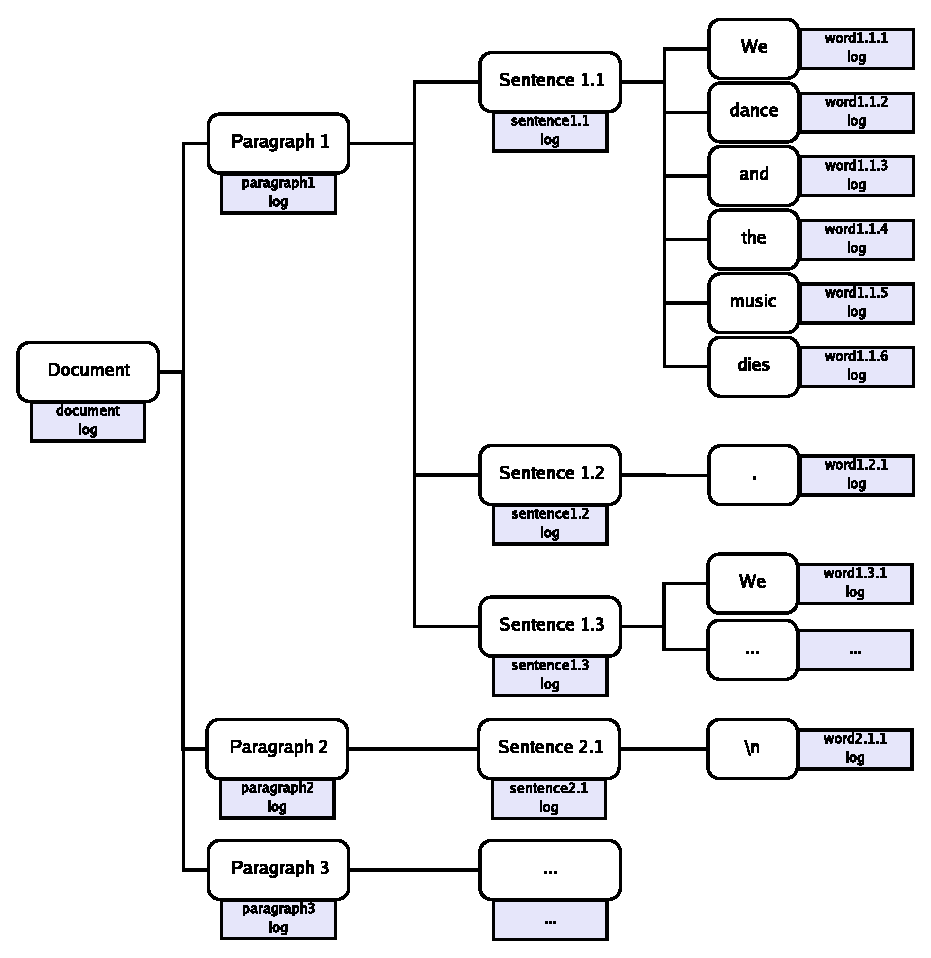
\includegraphics{img/treeex.eps}
\end{center}
\caption{Example of a document representation}
\label{fig:treeex}
\end{figure}

Figure \ref{fig:treeex} illustrates how the following document (formed of two paragraphs)
is represented in our structure:

\begin{center}
\begin{tabular}[c]{|l|}
\hline
We dance and the music dies.
We run through the stars.\\
We are without excuse.\\
\hline
\end{tabular}
\end{center}

\emph{Note: You might have noticed a difference from the model we have described previously, namely that
there are no nodes to represent characters. This is because in our implementation we tried to
save a bit of memory and not store each character as a separate object. We wanted to do this
because the character node itself does not store any additional information other than the character
itself (what we really mean is that there is no log associated with a virtual character node because
there are no operations which can be done at the character level, i.e. the operations with the finest
granularity in our model are the insertion and deletion of single characters, and these operations
pertain to the word level). Therefore, by simply making a few adjustments we were able to save quite
a bit of memory without any loss in generality. The fields whose interpretation we had to change
in order to achieve this were the \emph{content} and \emph{length}. Since level 4 nodes no longer
exist, the \emph{content} of level 3 - word - nodes was defined to contain a string which represents
all the characters in the node. The \emph{length} then also had to be adapted, so that the length
of level 3 nodes is now the length of the content string.}

Aside from that, figure \ref{fig:treeex} shows the hierarchical organization of the document and highlights
the log associated with each node. You can see that the root of the tree represents the document
itself. The document's children are the three paragraphs, each paragraph has the sentence that it
is formed of as children and so on. As you can see in the figure as well, the punctuation marks
are represented as nodes of their own. Each punctuation mark will be represented as a separate
paragraph, sentence or word (depending on the type of separator it is). This means that paragraph
separators will be represented as separate paragraphs, sentence separators (such as the '.' you
can see in the figure) will be represented as separate sentences and word separators will be
represented as separate words. In the case of paragraph and sentence separators, the entire
structure down to the word will be created (if you take the '.' in the figure, for example, you
can see that it forms a sentence on its own containing just one word; that word represents the
punctuation mark itself; another example of this is the paragraph separator, '$\backslash$n',
from the figure - notice how the entire structure down to the word is created).

This is the tree structure we shall be using to represent the text documents used in our project.

\section{Operations and operation transformation}

\subsection{Operation definition}
\label{sec:opdef}

Once the tree structure was defined, the next step was to devise a way in which operations
are represented in the system. Our model only uses two types of operations: insertion and
deletion. However, as we wanted to overcome some of the disadvantages mentioned in the previous
section, the operations allowed in our system are not only the classic insertion and deletion
of characters, but an extended set of these, consisting of the following operations:

\begin{itemize}

\item InsertChar and DeleteChar
\item InsertWord and DeleteWord
\item InsertSentence and DeleteSentence
\item InsertParagraph and DeleteParagraph

\end{itemize}

Besides these, a special type of operation was also added in order to specify a null effect:

\begin{itemize}

\item NOP

\end{itemize}

Formally speaking, all the nine operations listed above can be defined in the following
manner:

\begin{defi}

An \emph{operation} is a structure of the form $op=\{type,level,index,content\}$, where:

\begin{itemize}

\item \emph{type} represents the type of the operation, $type \in \{insert,delete,nop\}$.

\item \emph{level} represents the level in the tree to which the operation pertains,
      $level \in \{0,1,2,3\}$.

\item \emph{index} represents an array of indices, with $index[i]=$ the index for the
      $i^{th}$ level of the tree, $i \in \{0,\dots,level\}$.

\item \emph{content} represents the text content of the operation, i.e. the text inserted
      or deleted by the operation.

\end{itemize}
\end{defi}

The \emph{type} property defines whether the operation at hand is an insert, a delete
or a NOP. If the operation is a NOP none of the other fields are of importance. The
\emph{level} tells us if the operations is at the document (0) level (i.e. an InsertParagraph
of DeleteParagraph), at the paragraph (1) level (i.e. an InsertSentence or DeleteSentence),.
at the sentence (2) level (i.e. an InsertWord or DeleteWord) or at the word (3) level
(i.e. an InsertChar or DeleteChar). The \emph{index} gives us the position in the document
where we have to insert that particular unit of text. For instance, in the case of a
InsertChar, index will contain 4 entries with the following significance: index[0] gives
us the paragraph in which we want to insert the character, index[1] gives us the sentence
within the paragraph in which we want to insert the character, index[2] the word within
the sentence and index[3] the position in the word at which to insert the character.
Please notice that index contains exactly $level$ entries for each operations, where
$level$ is the actual level parameter of the operation. Finally, the \emph{content}
holds the inserted/deleted text (a character for InsertChar/DeleteChar, a word for
InsertWord/DeleteWord and so on).

For simplicity, in the explanations that follow, we shall denote operations by specifying
the type and the level in the operation name (i.e. InsertWord, DeleteParagraph, etc.), the
index as separate parameters (whose number depends on the level of the operation) and 
the content. An example would be \textbf{DeleteWord(2, 1, 5, ''hello'')}. In this case,
the operation type is insert, the operation level is 2 (sentence), the index is the array
[2, 1, 5] and the content is ''hello''. In order to avoid misunderstandings, please notice
that a DeleteWord operation is an operation at the sentence level (i.e. level 2), not at
the word level. This is because we insert and delete words into a particular sentence and,
therefore, the operations will appear in the log at the sentence level. This is why we say
they pertain to the sentence level. The same holds for all other types of operations as
well (InsertChar and DeleteChar pertain to the word level and so on).

\subsection{Applying operations}
\label{sec:applyop}

The first thing that needs to be explained about operations is the way they are applied
on the document structure in order to update it. The applying of an operation is necessary
in very different circumstances, ranging from executing local operations to  integrating
remote ones. As it is very important to understand how the document structure changes as
an effect of applying operation, we shall try to explain in this section how this is
achieved in our project.

Listing \ref{list:applyOp} reproduces a stripped down version of the code that implements
this. We shall try to walk through it line by line and explain the actions that are performed.
The first thing to notice is the parameters of the method. These are the operation that
has to be executed and a tree node. The method is always called from the outside using
the root of the document tree as the node. We say ``from the outside'' because, as the method is
recursive, when it calls itself recursively, values other than the root of the document
tree will be used.

\begin{lstlisting}[frame=lines,float=p,caption=apply operation,label=list:applyOp]
applyOperation(Operation op, DocumentTreeNode node)
{
	if (op.getType() == OperationType.nop)
		return;

	if (node.getLevel() == TreeLevel.document)
		childNo = op.index[0];
	else if (node.getLevel() == TreeLevel.paragraph)
		childNo = op.index[1];
	else if (node.getLevel() == TreeLevel.sentence)
		childNo = op.index[2];
	else if (node.getLevel() == TreeLevel.word)
		childNo = op.index[3];

	if (op.getLevel() != node.getLevel())
		applyOperation(op, node.getChildAt(childNo));
	else
	{
		if (op.getType() == OperationType.insert)
		{
			if (op.getLevel() == TreeLevel.word)
			{
				node.setContent(node.getContent().substring(0, childNo) +
					op.getContent() +
					node.getContent().substring(childNo));
			}
			else if (op.getLevel() == TreeLevel.sentence)
				node.addChildAt(childNo,
					Parser.parseWord(op.getContent()));
			else if (op.getLevel() == TreeLevel.paragraph)
				node.addChildAt(childNo,
					Parser.parseSentence(op.getContent()));
			else if (op.getLevel() == TreeLevel.document)
				node.addChildAt(childNo,
					Parser.parseParagraph(op.getContent()));
		}
		else if (op.getType() == OperationType.delete)
		{
			if (op.getLevel() == TreeLevel.word)
				node.setContent(node.getContent().substring(0, childno) +
					node.getContent().substring(childNo + 1));
			else
			{
				inverse(node.getChildAt(childNo));
				op.setContent(node.getChildAt(childNo).getContent());

				node.removeChild(childNo);
			}
		}
	}
}
\end{lstlisting}

The first thing to do is to check whether we are dealing with a NOP. If so, the method simply
returns as no changes have to be made to the document tree. If this is not the case, the
variable \emph{childNo} is assigned with a value depending on the level in the tree where the
\emph{node} parameter is. The idea is that we want \emph{childNo} to hold the number
of the child of the current node that the operation index indicates. This is used to
recursively go down the tree until the ``work node'' is reached. By ``work node'' we
refer to the node where the changes actually have to take place. If the operation is
an InsertWord, for example, the changes have to take place when we reach the sentence
level in the tree (i.e. reach the node that represents the sentence in which the word
has to be inserted). The assignment is done in the lines 6-13. Next, we check to see
whether we have already reached the level in the tree where we have to make the changes.
If we have not, a recursive call to applyOperation is made in order to go one level down
the tree (this is achieved by calling the method using the appropriate child of the
current \emph{node} as the second parameter).

Lines 19 through 35 show how an insert operation is executed. In a nutshell, if we are
dealing with an InsertChar (i.e. the level of the operation is the word level) all we
have to do is modify the content of the word node in order for it to contain the
inserted character in the position specified by \emph{index[3]}. If the operation
pertains to a level higher than the word level, we resort to one of the \emph{parseWord()},
\emph{parseSentence()} or \emph{parseParagraph()} methods, which will build the entire
subtree that correctly models the content to insert and return its root. This root
we add as a new child of the current \emph{node} in the position indicated by
\emph{childNo} (if you think about it, this is actually analogous to inserting a
single character at the appropriate position in the word for operations at the word
level).

Finally, lines 39 through 48 illustrate how a delete operation is handled. A delete
at the word level is executed by simply removing the indicated character from the
appropriate word (in a similar manner to the way an insert operation adds it), while
a delete at a higher level in the tree simply removes the child indexed by \emph{childNo}
from the current \emph{node}'s list of children (line 47 in the code). Lines 44 and 45
are necessary for local operations only in order for the content of the locally
generated operation to be correctly stored (even thought the inversion is executed for
remote operations as well, its effect is irrelevant in this case because the remote
operations, once executed locally, are discarded; even if we change the content
of the operation in line 45, since the operation is discarded anyway, this has no
further implications; moreover, since the operation is a delete, any changes that are
generated by the inverse method are lost anyway when the whole subtree is deleted
in 47). The \emph{inverse()} method called in
line 44 executes the inverse of all operations (insert instead of delete and
vice-versa) from the subtree it receives as parameter in the reverse order than
that in which they have been stored in the log. The purpose of doing this is to
ensure that whatever changes might have been done locally to the subtree to be
deleted are reversed. The reason for this is that these changes will be lost once
the subtree is deleted in line 47, but the content stored in the delete operation
would still reflect them, were we not to call the \emph{inverse()} operation. This
would lead to inconsistencies once the operation would be sent to other sites.
Once the \emph{inverse()} method is called, however, we can safely store the
content of the operation in line 45.

Now that the way operations are applied is clear, let us advance to the next important
operation-related functionality, namely the two basic transformations: the inclusion
and the exclusion transformation.

\subsection{Inclusion and exclusion transformation}

As you probably recall, the previous chapter introduced and explained the whole
concept of inclusion and exclusion transformations in the theoretical context
in which they originally appeared. In this section we assume that the reader is
already accustomed with the concepts already described in chapter \ref{chap:incexcl}
and go on to describing the way we put these concepts into practice in our project.

We have based our development of the transformation functions on the close of analysis
of \cite{imine03}, which verifies the correctness of state-of-art transformation
functions defined on strings using an automated theorem prover, in order to avoid
the common mistakes others have made when writing such functions.

\emph{Note: For the remainder of this section we make the following naming convention:
from the two operations involved in an inclusion/exclusion transformation we denote
the operation that has to be transformed as the \emph{current operation} and the
operation against which the current operation has to be transformed as the
\emph{against operation}.}

We start our discussion by mentioning that we had to define the transformations
in a way that takes into account the fact that the operations are no longer applied
on a linear structure, but on a hierarchical one. Several implications follow from here,
such as the fact that the inclusion/exclusion of an against operation that refers
to lower level of the tree than that the current operation refers to has no effect whatsoever.
This is also the case with two operations on the same level, but referring to
units which are not the children of the same parent. However, an against operation
at a higher level in the tree than the current operation might need to change the
appropriate index value in the current operation (when the two operation refer to
the same subtree).

This approach is rather different than that in use by linear systems, where any
against operation that refers to a position before that of the current operation
is sure to change the index of the current operation. Herein lies one of the advantages
of using a tree-based representation: significantly fewer operation will have to
be changed.

The inclusion and exclusion transformations we explain in this section represent
the building blocks of higher level functions the algorithm uses, therefore their
understanding is essential for a good comprehension of the algorithm later on.

Both the inclusion and the exclusion methods are part of the Operation class, therefore
all the methods that are not used within are themselves members of the Operation class.

\subsubsection{The \emph{include} method}

We shall start with the \emph{include()} method which is displayed in listing \ref{list:include}.

\begin{lstlisting}[frame=lines,float=p,caption=include operation,label=list:include]
Operation include(Operation opAgainst)
{
	Operation result = clone();

	if (opAgainst.getType() == OperationType.nop ||
		getType() == OperationType.nop)
		return result;

	// the level of the current operation
	int levelCurrent = getLevel();
	// the level of the against operation
	int levelAgainst = opAgainst.getLevel();

	if (levelAgainst > levelCurrent)
		return result;

	for (int i = 0; i < levelAgainst; i++)
		if (index[i] != opAgainst.index[i])
			return result;

	if (opAgainst.getType() == OperationType.delete)
	{
		if (index[levelAgainst] == opAgainst.index[levelAgainst])
			if (levelCurrent != levelAgainst ||
				levelCurrent == levelAgainst &&
				getType() == OperationType.delete)
				result.setType(OperationType.nop);

		if (index[levelAgainst] > opAgainst.index[levelAgainst])
			result.index[levelAgainst]--;
	}
	else if (opAgainst.getType() == OperationType.insert)
	{
		if (index[levelAgainst] == opAgainst.index[levelAgainst] &&
			getType() == OperationType.insert &&
			levelCurrent == levelAgainst)
			
		{
			if (current and against ops generated at different sites)
			{
				if (getContent() > opAgainst.getContent())
					result.index[levelAgainst]++;
			}

			if (current and against ops are the same operation)
				result.setType(OperationType.nop);
		}
		else if (index[levelAgainst] >= opAgainst.index[levelAgainst])
			result.index[levelAgainst]++;
	}

	return result;
}
\end{lstlisting}

Let us walk through the code one step at a time and see what happens. The first
thing to do is clone the current operation in order to obtain a version of it
(initially identical) which we can then modify. A check is then made in order to
find out whether or not either of the two operations in question (the current or
the against operation) is a NOP. If this is the case, we can simply return since
an operation does not change by including a NOP and a NOP does not change by
including an operation, whatever it is.

Once this is out of the way, the next thing to do is obtain the level at which
each of the two operations refer and store it in \emph{levelCurrent} and
\emph{levelAgainst}. The level an operation refers to is given by its type.
An InsertParagraph, for instance, acts at level 0 in the tree, while a DeleteChar
acts at level 3.  Next, a few checks are made in order to see if the against
operation should have any effect on current operation. First, if its level
is lower than that of the current operation, we can safely return from the
method without making any changes to the current operation since, for example,
an InsertWord cannot influence a DeleteSentence in any way, even if it is in
that exact sentence. This is because the only index an InsertWord would influence
would be the word index, but a DeleteSentence does not have a word index in the
first place, so there is nothing to influence. Then, we want to see whether the
two operations refer to the same subtree (\emph{Note: two operations refer to
the same subtree if the nodes they work on to are either identical (i.e. they refer
to the same node) or if one is the ancestor of the other}). This is achieved in
lines 17-19. The idea here is that if the against operation is an InsertSentence
and the current operation is a DeleteWord that InsertSentence could only influence
the sentence index of the DeleteWord \emph{if} the word is deleted from a sentence
that is in the same paragraph as the one to which the InsertSentence is referring.

At this point of execution we know that the against operation might actually
have an effect on the current operation. If the against operation is a \emph{delete}
there are two cases in which the current operation needs to be changed.

The first case is actually a combination of conditions, the first of which requires
that the lowest available index of the against operation (i.e. the index
which corresponds to the actual level of the tree to which the against operation
refers) is equal to the corresponding index in the current operation. These means
that both operations work on the same node or that the current operation works on
a node that is the subtree the root of which is the node the against operation
works on. Further on, we need to consider the two cases separately.

\begin{itemize}
\item when the current operation is of a lower level than the against operation,
      no additional condition has to be met. This translates to the fact that
      the against operation is actually deleting the entire subtree in which the
      node the current operation works on is located. Obviously, the object of
      the current operation ceases its existence once the against operation is
      executed, so the current operation no longer has a purpose, therefore it
      needs to be canceled.
\item when the two operations refer to the same level, the current operation also
      has to be a delete. This translates to the fact that both operations are
      effectively deleting the exact same semantic unit (may it be paragraph, a
      sentence, a word or a character). It is clear that in order to preserve the
      intention of both users the deletion only has to be performed once. The solution
      is again to cancel the current operation, since the against operation already
      did its job.
\end{itemize}

So, in both of these two cases, the current operation needs to be changed to a
NOP, which is exactly what line 27 does.

The second case to consider is more straightforward and it represents the typical
inclusion case, and it is analogous to that used in linear systems. If the index of the current
operation corresponding to the level of the against operation is greater than the
one of the against operation, then it is clear that it has to be decreased by one
since the against operation deleted a node. Therefore, the node the current operation
index was originally referring to is now one position more to the left. This case
is covered in lines 29-30.

Now let us see what happens when the against operation is an \emph{insert} operation.
Again, we have two cases to deal with.

The first case is when the lowest available index of the against operation (that
corresponding to the actual level of the tree to which the against operations refers)
is equal to the corresponding index in the current operation \emph{and} both operations
refer to the same level of the tree \emph{and} the current operation is also an insert.
As before, this means that both operations insert a semantic unit (a character, a word, etc.)
at the same index of the parent node. The discussion here is a bit more difficult.
On one hand we have the case when the two operations were generated by different
sites (see line 39). In this case it is irrelevant what order the two semantic units are
inserted in (since no priority exists in what the two users who generated the two
operations are concerned, any order of insertion is as good as the other), but it is
essential that they are inserted in the same order on all sites. In order to achieve
this, a simple trick was employed, namely to alphabetically compare the two contents
to be inserted and always insert the content which is alphabetically ``lower'' before
the content that is alphabetically ``higher''. This means that if the against operation
inserts the ``lower'' content, then the current operation has to have its index increased
by 1 so that the insertion it makes takes place in the position immediately after the one
on which the content of the against operation was inserted. It would have been equally
correct to increase the index had the opposite case been true (i.e. if the against
operation inserted the ``higher'' content). On the other hand, we
have the case when the two operations were generated by the same site. In this case
no reordering has to be made since the two operations were generated by the same user
and the original order has to be kept.

An additional check is then made to see if the two operations have the same unique
identifier (line 45). If it is true, then the current operation is canceled (i.e. turned
to NOP). This case can appear when direct user synchronization is used. We shall
return to it when we talk about this facility of our application.

Again, the second case is the ``classical'' one, analogous to that used in linear
systems. If the index of the current operation corresponding to the level of the
against operation is greater than or equal to that of the against operation, it has
to be increased by one since the against operation inserted a new node. Therefore, the node
the current operation index was originally referring to is now one position more to
the right. This case is covered in lines 48-49.

At the end, the transformed version of the current operation is returned.

\subsubsection{The \emph{exclude} method}

Now, we go on to explaining the way in which the exclusion of an operation is
achieved in our algorithm. You can find the method illustrated in listing
\ref{list:exclude}.

\begin{lstlisting}[frame=lines,float=p,caption=exclude operation,label=list:exclude]
public Operation exclude(Operation opAgainst)
{
	Operation result clone();

	if (opAgainst.getType() == OperationType.nop ||
		getType() == OperationType.nop)
		return result;

	// the level of the current operation
	int levelCurrent = getLevel();
	// the level of the against operation
	int levelAgainst = opAgainst.getLevel();

	if (levelAgainst > levelCurrent)
		return result;

	for (int i = 0; i < levelAgainst; i++)
		if (index[i] != opAgainst.index[i])
			return result;

	if (opAgainst.getType() == OperationType.insert)
	{
		if (index[levelAgainst] == opAgainst.index[levelAgainst])
		{
			if (levelCurrent != levelAgainst ||
				levelCurrent == levelAgainst &&
				getType() == OperationType.delete)
				result.setType(OperationType.nop);
		}

		if (index[levelAgainst] > opAgainst.index[levelAgainst])
			result.index[levelAgainst]--;
	}
	else if (opAgainst.getType() == OperationType.delete)
	{
		if (index[levelAgainst] >= opAgainst.index[levelAgainst])
			result.index[levelAgainst]++;
	}

	return result;
}
\end{lstlisting}

The \emph{exclude} method is slightly more straightforward than the include one.
The first lines are roughly identical. Here, as in the case of the include method,
excluding NOP from an operation or excluding an operation from NOP has no effect
whatsoever, so we can simply return. Next, we also need to retrieve the level at
which each of the two operations works and store it into two variables which we
have named the same for convenience.

Once again, if the against operation refers to a lower level than the current operation
or if the two operations refer to different subtrees (i.e. the nodes they refer to
are neither the same nor is any of them the ancestor of the other), there is nothing that
we have to do and can simply return. For a more elaborate discussion about this,
please refer to the previous subsection where we explain the include method.

Next, let us see what happens when the against operation is an insert. As with include,
we have two cases. The first one arises when the indices of the two operations that indicate
the position at the level at which the against operation has effect coincide.
This means that they either refer to the same node of the document tree or that the
current operation refers to a node that is in the subtree the root of which is the node
the against operation acts on. If the former is the case and the current
operation is itself a delete operation, it means that the current operation deletes
the exact same node the against operation inserts. Excluding the effect of the against
operation is just another way of saying that we need to see what happens with the current operation
when the against operation is no longer executed. Obviously, if the node is no longer
inserted, it cannot be deleted by the current operation, so the operation has to be
canceled altogether. In the latter case (of the two cases described above), the current
operation wants to insert or delete a node in/from the subtree that has been inserted
by the against operation. But if the insertion no longer takes place, the current
operation (regardless of whether it is an insert or a delete) does not makes sense
anymore, so again it has to be canceled. This is what we do in line 28.

The second case appears when the index of the current operation that gives the positioning
in the level the against operation refers to is greater than its counterpart in the
against operation. We need to decrease the mentioned current operation index by one
since the node it indicates moves one position to the left if the against operation
(which, if you remember, was an insert) is no longer executed. For the sake of symmetry,
let us mention that this is the ``classical'' case.

Finally, when the against operation is a delete, we only have to deal with the
``classical'' case and increase the index of the current operation that indicates the
position in the level the against operation refers to by one if the condition in
line 36 is met (this is the same condition that we have described over and over in the
previous paragraphs, so chances are that you are already familiar with it). The reason
we have to add 1 to the index is that if the delete operation is no longer executed,
the node the index indicates moves one position to the right.

As in the case of the include method, we terminate the method by returning the modified
version of the current operation.

\subsection{Transpose and symmetric inclusion transformation}
\label{sec:transp}

The final step before introducing the merging algorithm itself is to define two additional
functions which ``wrap'' the inclusion and exclusion transformation in order to obtain
the form in which the algorithm actually uses them. These two functions are \emph{transpose}
and \emph{symmetric inclusion transformation}.

The \emph{transpose} operation is defined to transpose $O_{a}$ and $O_{b}$ where $O_{a} \mapsto
O_{b}$ in order to achieve $O_{b} \mapsto O_{a}$ (see definition \ref{def:cprec} if you have
forgotten what ``$\mapsto$'' stands for). Therefore, if $O_{k-1} \mapsto O_{k} \mapsto
O_{k+1}$, after \emph{transpose($O_{k},O_{k+1}$)}, it becomes $O_{k-1} \mapsto O_{k+1} \mapsto
O_{k}$. As a result, $O_{k+1}$ can be executed right after $O_{k-1}$. This is exactly what
we shall use transpose for: take operation $O_{k}$ from the log and move it (transpose it)
successively to the right in order for it to become the last operation of the log. But we
shall talk about this later.

For now, we need to explain why a simple inversion of $O_{a}$ and $O_{b}$ would not suffice.
The problem is that if we reverse the order of execution of the two operations there are
some changes that we have to make to the operations in order for user intention to be preserved.
These changes are rather intuitive. First we have to make sure that operation $O_{b}$
excludes the effect of operation $O_{a}$ since if we are moving it before $O_{a}$ it means
that the effect of $O_{a}$ (which is initially included in $O_{b}$) has to be canceled.
Second, we have to make sure that the effect of $O_{b}$ is included into $O_{a}$. This is
because the transpose implies that $O_{a}$ will be executed after $O_{b}$, so it should
become aware of its effect (since it initially was not as it was executed before it).
Putting this into code, what we obtain is:

\begin{center}
\begin{tabular}[c]{|l|}
\hline
\emph{Transpose($O_{a},O_{b}$)}\\
\textbf{\{}\\
\verb+    +$O := ET(O_{b},O_{a})$;\\
\verb+    +$O_{b} := IT(O_{a},O)$;\\
\verb+    +$O_{a} := O$;\\
\textbf{\}}\\
\hline
\end{tabular}
\end{center}

\noindent{}where by $IT$ we denote the \emph{inclusion transformation} and by $ET$ we
denote the \emph{exclusion transformation}. The actual implementation is slightly more
complicated because several special cases have to be taken into consideration.

One of them is the case when $O_{a}$ is an insert on a specific position and $O_{b}$
is a delete from the same position. If you think of how the include and exclude operations
are implemented, you realize that if we simply execute the transpose in the above form
we would first exclude the effect of $O_{a}$ (the insert) from $O_{b}$ (the delete). This
would yield a NOP since otherwise $O_{b}$ would end up trying to delete something that
doesn't exist yet. Transforming $O_{b}$ into a NOP would be perfectly fine. The problem
comes at the next step when we include the effect of the NOP in $O_{a}$. Including $O_{a}$
against a NOP yields an unmodified $O_{a}$ as a result. This is obviously wrong since the
effect of applying the modified $O_{b}$ and $O_{a}$ (in this order) after the transpose
should be the same as applying the original $O_{a}$ and $O_{b}$ (in this order). Clearly,
this does not hold if $O_{b}$ becomes NOP and $O_{a}$ remains unchanged. In order to find a
solution for this particular case we had to handle it separately and transform both
$O_{a}$ and $O_{b}$ to NOP.

Another special case appears when $O_{a}$ and $O$ (the version of $O_{b}$ which no longer
contains the effect of $O_{a}$) are both Insert's in the same position. For example,
consider the case when $O_{a}=InsertChar(3,1,2,0,\text{'a'})$ and $O_{b}=InsertChar(3,1,2,1,\text{'b'})$.
The final string that would be obtained is ``ab''. After excluding the effect of $O_{a}$
from $O_{b}$ (in line 1 of the transpose), the new version of $O_{b}$ would be
$O=InsertChar(3,1,2,\textcolor{red}{0},\text{'b'})$. If now we were to simply perform
the inclusion of $O_{a}$ against $O$ (the second line of the transpose operation), $O_{b}$
would be assigned $O_{b}=InsertChar(3,1,2,\textcolor{red}{1},\text{'a'})$.
The final result would be wrong because the effect of applying the modified $O_{b}$
and then the modified $O_{a}$ (which is what we would do after the call to transpose) would be
the obtaining of the string ``ba'' instead of the initial string, ``ab''. In order
to solve this special case we need to replace line 2 of the transpose function
(for this case only) with $O_{b} := O_{a}$ (meaning that we are assigning $O_{a}$ to
$O_{b}$ as is, without the inclusion of the effect of $O$). The result of this in the
case we were discussing above is that we would eventually obtain
$O_{b}=InsertChar(3,1,2,\textcolor{red}{0},\text{'a'})$, which means that by
executing the modified form of $O_{b}$ and then of $O_{a}$ we would obtain
the correct string, ``ab''.

However, once all these special cases are dealt with, the procedure behaves correctly
and achieves what we wanted in the first place: given two operations, $O_{a}$ and $O_{b}$
such that $O_{a} \mapsto O_{b}$ the transpose function changes them so that afterwards
$O_{b} \mapsto O_{a}$. More than that, if the new $O_{b}$ and $O_{a}$ are executed in
this order, they will achieve the same effect as the execution of the original
$O_{a}$ and $O_{b}$ (in this order).

The second operation we were mentioning at the beginning of this section was the
\emph{symmetric inclusion transformation}. Let us start with the following example
in order to clarify why the symmetric inclusion transformation is needed. Imagine
the simple scenario of two users (John and Mary) on two different sites working
on the same version of a document. Assume each of them performs just one operation
(John performs operation $O_{J}$ and Mary operation $O_{M}$) on his/her working copy.
Then, Mary commits her operation to the repository. John has to update his local copy
of the document before being able to commit himself. Let us analyze what happens
during this update. John will receive a single operation from the repository, $O_{M}$,
which has to be integrated into his version. The operation cannot be executed 'as is' because
the context John currently has is different from the context in which $O_{M}$ was
generated. Therefore, $O_{M}$ has to include the effect of $O_{J}$ for a correct execution.
Once this is accomplished, $O_{M}$ can be safely
executed on John's local copy. The question that remains unanswered is: what will
John commit to the repository? He cannot simply commit $O_{J}$ as it is because
the version on the repository has changed (meaning that the context on the repository
is now different from the one in which $O_{J}$ was generated). The solution is
to make $O_{J}$ include the effect of the operation on the repository (namely, the
effect of $O_{M}$). Once this is done, the modified version of $O_{J}$ can be safely
committed to the repository since now its context corresponds to that on the repository.

If we take a second and think back about the operations we have done, we shall realize
that they were two include operations. First, we included the effect of $O_{J}$ in
$O_{M}$ and then we included the effect of $O_{M}$ into $O_{J}$. As you have probably
figured out on your own already, this is a \emph{symmetric inclusion}. Even though
the real case will be slightly more complicated than the one from above, still the
symmetric inclusion transformation will have to be used in that exact same way on
individual pairs of local and remote operations. The procedure itself, as you
might imagine, is very straightforward:

\begin{center}
\begin{tabular}[c]{|l|}
\hline
\emph{SymmetricInclusion($O_{a},O_{b}$)}\\
\textbf{\{}\\
\verb+    +$O := IT(O_{a},O_{b})$;\\
\verb+    +$O_{b} := IT(O_{b},O_{a})$;\\
\verb+    +$O_{a} := O$;\\
\textbf{\}}\\
\hline
\end{tabular}
\end{center}

This being said, we now have all the background laid out and are finally ready to advance
to the description of the commit, update and checkout procedures themselves.

\section{The stages of the collaborative editing algorithm}

As we explained in section \ref{sec:cmm}, the main operations of an asynchronous editing
system are the commit, update and checkout operations. As ours is precisely such a system,
we also had to offer an implementation of the three basic operations. This was actually
the most consistent and challenging part of the project. In this section we shall describe
the way in which we have implemented each of the above operations.

\subsection{The commit stage}
\label{sec:commit}

To commit a working copy in the repository, a certain course of actions has to be taken in
order to ensure the consistency of the system. We describe this course of actions as a sequence
of steps the system executes when the user requests that the document (s)he has changed locally
be committed to the repository.

The first action the system performs is send a message to the repository including the version
number of the document which is the base version for the editing session (i.e. the latest version
of the document that is integrated in the local working copy of this user). This is done
in order to find out whether the current version on the repository is identical to the base
version of the current user. The repository does this check and sends a positive or negative answer
back to the user. Let us analyze what each of these cases means.

If the current version on the repository is identical to the base version of the
user, it means that no changes have been committed to the repository that this user is not aware
of. Therefore, the user can simply send his log to be stored on the repository as is,
without any modifications. If, however, the repository answers that its current version is
different from the base version of the user, it means that somebody else has committed some
changes that this user is not aware of. Consequently, the user cannot simply send his unmodified
local log to the repository. This is because the operations would end up to be executed in
a different context than the one in which they were generated, leading to erroneous results.

To better understand this, think of the following concrete case: when the user starts working
the version on the repository is $V_{k}$. This will become his base version. Suppose he would
only execute one operation, $O$. The context of this operation is version $V_{k}$ of the document.
In the meantime, the repository's version changes (by other users committing their own changes)
from $V_{k}$ to $V_{k+n}$. And now assume that $O$ was committed as is on the repository. Later,
when another user would check out the document from the repository, (s)he would receive a set
of operations which includes $O$, which (s)he would execute in the order in which (s)he receives
them. This means that $O$ would end up executed in the context of version $V_{k+n}$ which is
different from the one it was generated in ($V_{k}$). The effect is that the user intention would
probably be not preserved.

In light of these explanations, it is hopefully clear why we cannot simply commit an unchanged
log to the repository when the base version on the local site and the current version of the
repository differ. What happens in this case is that the system will warn the user that his/her
version of the document needs to be updated before (s)he can successfully commit and then stop
the commit stage. In order to update the document, the update procedure has to be called. What
this procedure does is described in the next section. Once the update is complete, the user
can try to commit once again by recalling the commit procedure, thus re-initiating the same
sequence of actions from above.

Now, let us see what happens when the repository sends back a positive answer and the user can
carry on with the commit. The user should send the local log to be stored on the repository.
What we need to detail here is what the local log actually is in our case, given
the fact that we have a log distributed throughout the tree that represents the document. Figure
\ref {fig:clog} gives you an overall image of how this is done. What you see in this figure is
a sample document tree in which the (possibly empty) log of each node is shown.

\begin{figure}[!p]
\begin{center}
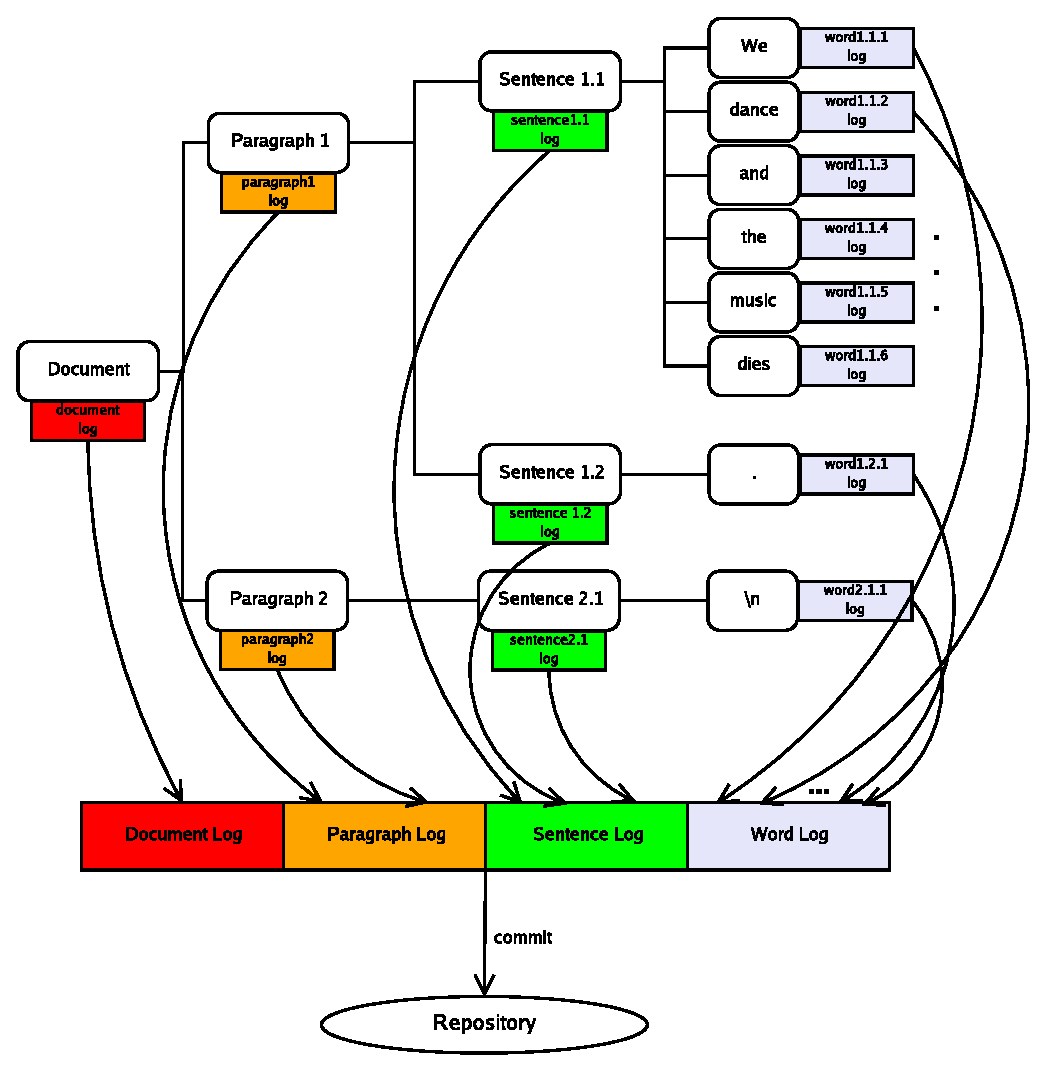
\includegraphics{img/commit.eps}
\end{center}
\caption{The committed log}
\label{fig:clog}
\end{figure}

The figure depicts how the serialized log that is sent to the repository is composed. The first
operations will be those in the document log, then those in the paragraph logs (with paragraph
1 log first, paragraph 2 log second and so on), then those in the sentence logs (ordered
corresponding to the numbering in the figure) and, finally, those in the word logs. In fewer
words, the commit log is composed by doing a breadth-first traversal of the document tree
and orderly adding the log associated with each node to the commit log. What we obtain is
a log in which all document level operations come first, all paragraph level operations
(ordered by paragraph number) come second, all sentence level operations (ordered by
sentence number) come third and all word level operations (ordered by word number) come
last.

This ordering is not random. The reason for which we have ordered the operations this way will
become more obvious when we explain the update stage. A short explanation would be that when,
during the update stage, we merge the log from the repository with the local log, we need to
progressively update the local tree in a top-down manner, in order for the level $k$ to
already be updated when we merge operations on level $k+1$ and below. If it were not so,
we would have no way of knowing what \emph{local} $k$-level node operations acting on the
$k+1$ and lower levels from the \emph{remote} log refer to. In other words, if a remote operation's
$k$-level index is $m$ (while the operation itself refers to level $k+1$ or below), if we
do not update the \emph{local} level $k$ of the tree before executing the operation, we
do not know which \emph{local} node on level $k$ is actually the $m^{th}$, so we basically
do not know which $k$-level logs to merge.

Once this commit log is generated, all that remains to be done is to send it to the repository.
Of course, it could be the case that between the initial comparison of the local base version
and the current version on the repository, the situation has changed and the two versions might no
longer be the same when the commit is actually attempted. In order to ensure that a faulty
commit does not take place, the base version is once again sent along with the commit log,
thus allowing the repository to atomically redo the comparison and, if successful, to commit
the changes. If, however, the version on the repository has changed, a failure message will
be sent back to the client telling it that it needs to update its version before committing.
The client would then have to do an update and then restart the whole commit procedure.
If the version has not changed, then the changes are stored on the repository and the current
version number is increased by one.

All the client has to do in the case that it receives a positive response from the repository is
to empty the local log (since the operations it contained are now on the repository). This
is done by traversing the whole document tree and deleting all the logs associated with the
tree nodes. Also, the base version on the client is increased by one (the client is
aware of the changes which comprise the new version on the repository since it itself has
generated and committed those changes).

\subsection{The update stage}
\label{sec:update}

We have finally reached the most complex part of our algorithm, the update stage. In this
section we shall try to explain it as clearly as possible since it represents an essential
part of our work at this project. A necessary precondition for the thorough understanding
of this section is that you have worked your way through this entire chapter as all the concepts
and functions described previously are used in the implementation and we shall assume that you
are already familiar with them.

We shall break the description of the update method in two distinct parts and explain them
separately. These two parts are the basic merge algorithm (which takes two lists of operations,
merges them according to a series of rules and returns two transformed lists) and the actual
update algorithm which uses the merge algorithm internally in order to update the local
document tree with a log taken from the repository.

\subsubsection{The basic merge algorithm}
\label{sec:merge}

The basic merge algorithm we describe here is an adaptation of the one presented in \cite{shen02}.
In linear systems, this algorithm can be used 'as is' as the entire update stage since what it does
is merge two list of operations: the local log and the log from the repository. In a liner system
all we have is these two lists which contain all the operations. However, in our case it will need
to be integrated into a larger scale algorithm that traverses the local tree and the remote log of
operations in parallel and decides what sets of operations have to be compared and merged.

The reasons for which we need to merge the two lists should be already clear from the previous
sections, so we shall only lightly address them here. Basically, the local user has started working
from version $V_{k}$ on the repository. This is the last version which (s)he is aware of (i.e.
any operation that appears in versions higher than $V_{k}$ are unknown to this user). When (s)he
finishes editing and wants to commit the changes to the repository, the commit can be performed only
if the context of the local operations is modified so that it no longer is version $V_{k}$, but version
$V_{k+n}$ (the current version on the repository). In order to modify this context of the local
operations we need to take the operations that represent the delta between version $V_{k}$ and
version $V_{k+n}$ on the repository (in what follows we shall call these operations the
\emph{remote log}) and perform two actions:

\begin{itemize}
\item change the form of all the local operations to make them include the effects of the
      operations in the remote log (in other words, change the context of all local operations
      from version $V_{k}$ to version $V_{k+n}$)
\item apply the operations from the remote log on the local copy of this user in order to
      update it to version $V_{k+n}$. The operations, however, cannot be executed in the
      form in which they are received from the repository because the local context differs
      from the remote context in which these operations were generated. Consequently, they
      have to be transformed in order to include the effect of all the local operations before
      they can be executed
\end{itemize}

These two actions are achieved by the merge algorithm. Before advancing to the algorithm itself,
let us introduce two functions that we shall use. The first of them is called \emph{semantic
conflict}. In \cite{dourish96}, the conflicts are classified as being either syntactic or
semantic. Syntactic conflicts occur at the system infrastructure level, while semantic conflicts
are inconsistencies from the perspective of the application domain. In the case of the multi-user
text editing, consistency from the users' perspective is often not the same as consistency from
that of the system's. Generally, the operational transformation algorithms solve the syntactic
inconsistency problems, but they do not enforce semantic consistency. In \cite{munson94} and
\cite{shen02} an additional abstraction layer which would allow algorithm writers to completely
separate the syntactic merging rules form the semantic merging ones is thus introduced by means
of the semantic conflict function.

Generally speaking, a semantic merging policy is specified as a set of Semantic Merging Rules
(SMR) with which the \emph{Semantic-Conflict(SMR,$O_{r}$,$O_{l}$,CT)} determines whether two
concurrent updates, $O_{r}$ and $O_{l}$, are semantically conflicting according to the context
\emph{CT} on which they were generated. On one extreme, the function could automatically return
\emph{true/false} without human intervention if the \emph{SMR} has been well formulated. Automatic
detection of conflicts is the most desirable way. However, this is not at all easy to achieve.
On the other extreme, the detection of conflicts could be completely manual if the \emph{SMR} is
unable to be formulated in any way. As a result, it is completely up to the user to determine
what updates made by another user should be merged into his/her working copy, possibly with
consultation with that user. Manual detection of conflicts is the most general way for all
applications, although it is the least desirable way. In most cases, the detection of conflicts
is the combination of automatic and manual detections. In other words, some conflicts can be
automatically detected while others have to be detected by humans \cite{shen02}.

In our project, we took a rather simple approach to this issue and defined conflicts in the
following way: two operations are conflicting if they change the same semantic unit, where
the semantic unit is indicated by the working granularity level chosen by the user.
The user can decide if (s)he wants to work at the word, sentence or paragraph level. If the
user chooses, say, to work at the word level, it means that two concurrent operations changing
the same word will \emph{always} be conflicting. In order to achieve this, we provide the
following implementation of the \emph{semantic conflict} function:

\lstset{linewidth=340pt}
\begin{lstlisting}
boolean semanticConflict(Operation op1, Operation op2)
{
	if (op1.getType() == OperationType.nop ||
		op2.getType() == OperationType.nop)
		return false;

	if (level <= op1.getLevel())
	{
		for (int i = 0; i < level; i++)
			if (op1.getIndex()[i] != op2.getIndex()[i])
				return false;
				
		return true;
	}
	else
		return false;
}
\end{lstlisting}
\lstset{linewidth=450pt}

The two operations received as parameters are the two concurrent operations about which we need
to say whether they are conflicting or not. The \emph{level} variable that appears in the
code is the global variable set by the user. This is how the user makes his/her choice of
semantic unit (s)he wants to work on. A value of 4 for the level variable, for example,
indicates that the user wants to work at the word level. A precondition for calling this function
is that the two operations have to have the same level. Since it is only called from the
merge method where only operations of the same level are compared, this precondition is
always met. Another required precondition is that the context of the two operations is
the same. This is also ensured by the merge method.

The first thing the function does is check if any of the operations is a NOP. If this is
the case, it simply returns false since a NOP is never in conflict with any other operation.
Further on, the level the user chose to work at is compared with the level of the operations
(remember one of the preconditions said that the two operations need to be of the same level).
If the operations are of higher level than the level of conflict then false is returned (line
16) since they are not conflicting (for example, if the level is set to word level and the
two operations are insertion and deletion of, say, sentences, they are obviously not conflicting).
If, however, they are of the same level or of lower level than the level of conflict set by the
user, we need to check whether all their indices down to the level of conflict coincide. If so,
we conclude they are conflicting and return true (line 13). Otherwise, if any of the indices
down to the defined conflict level are different, false is returned (line 11) meaning that the
two are not conflicting (they refer to different semantic units).

This is the \emph{semantic conflict} implementation we shall use in the merge algorithm.

The second function we need to define is the \emph{remove operation} function. Its purpose is
to move an operation from position $i$ in a log on the last position in the log by transposing
(see \ref{sec:transp}) it one step at a time over operations $i+1$ through $n$. This function
will be used when an operation from the remote log is conflicting with one from the local
log and needs to be removed from the log. It cannot be simply removed since its effect has
to be excluded from all the operations that come after it in the log. Therefore, we need this
special \emph{remove operation} function which achieves this. Its implementation is rather
straightforward and it looks like this:

\lstset{linewidth=340pt}
\begin{lstlisting}
Operation removeOperation(int k, ArrayList log)
{
	for (int i = k; i < log.size() - 1; i++)
		Operation.transpose(log.get(i), log.get(i+1));

	return log.remove(log.size()-1);
}
\end{lstlisting}
\lstset{linewidth=450pt}

Lines 3-4 achieve the transposing of the operation at the end of the log, while line 6 removes
the transposed operation from the log and returns it.

Now that these two functions are clarified, we can go on to presenting the basic merge
algorithm. Figure \ref{fig:merge} shows what the merge operation is supposed to do. This is the case
when we would be dealing with a linear representation of the document. In our case, the situation
(as we mentioned) is slightly different, meaning that we would not compare the two logs directly,
but split them taking the tree structure into account and repetitively call the merge function.

\begin{figure}
\begin{center}
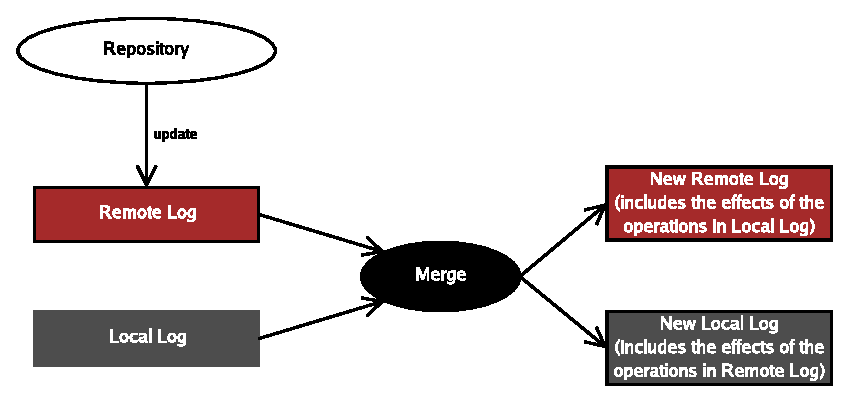
\includegraphics{img/merge.eps}
\end{center}
\caption{Merging two logs}
\label{fig:merge}
\end{figure}
 
As the figure shows, the input parameters of the merge operation are two logs, a remote and a local
one, and the output parameters are also two logs, the modified local and the modified remote log, each
of them changed in order to include the effects of the operations in the other one. The merge procedure
itself is illustrated in listing \ref{list:merge}.

\begin{lstlisting}[frame=lines,float=p,caption=the merge procedure,label=list:merge]
public void merge(ArrayList remoteLog, ArrayList localLog,
	ArrayList newRemoteLog, ArrayList newLocalLog)
{
	for (int i = 0; i < remoteLog.size(); i++)
	{
		// save local log into CLL
		ArrayList CLL = localLog.clone();

		// save operation on position i in remote log into CRLi
		Operation CRLi = remoteLog.get(i).clone();

		for (int j = 0; j < localLog.size(); j++)
		{
			if (semanticConflict(remoteLog.get(i), localLog.get(j)))
			{
				// restore remoteLog[i] from CRLi
				remoteLog.set(i, CRLi);

				// restore localLog from CLL
				localLog = CLL;

				// remove operation i from the remote log
				Operation o = removeOperation(i, remoteLog);
				i--;

				// add the inverse of the removed
				// operation to the local log
				newLocalLog.add(o.invert());

				// end the for loop
				break;
			}
			else
			{
				symInclusion(remoteLog.get(i), localLog.get(j));
			}
		}

		if (j == localLog.size())
		{
			newRemoteLog.add(remoteLog.get(i));
		}
	}

	for (int i = 0; i < localLog.size(); i++)
	{
		newLocalLog.add(localLog.get(i));
	}
}
\end{lstlisting}

In the way in which we apply the general update algorithm, whenever we call the merge function there
will be a current node which we shall have reached in our traversal of the tree. All operations from the
remote log and from the local log (the ones we use as actual parameters when calling the merge function)
will refer to that particular node. Thus, the \emph{remoteLog} contains a list of remote operations
that pertain to the current node (i.e. if the current node is a sentence, then the remote log will
contain any operations that insert or delete words in that particular sentence and nothing else -
neither of higher nor of lower levels). The \emph{localLog} contains the local operations that refer
to that node in the tree. The \emph{newRemoteLog} is the list of operations that should be executed
sequentially on the current document state of the working copy in order to update it. It will contain
most or all the operations from the original remote log, modified in order to include the effects of
those in the local one. We say that it might not actually contain all of the operations in the
original remote log because some of them might be in conflict with the local ones and would then
have to be removed. The \emph{newLocalLog} will store the list of operations which will have to replace
the local log pertaining to the current node. They will represent most or all the operations in the
local log transformed in order to include the ones in the remote log. Additionally, it might also
include the inverse of some of the operations in the remote log. Why this might be will become clear
soon.

The largest part of the function takes place within the big for loop (lines 4-43) which iterates over
the operations in the remote log. Thus, for each operation in the remote log we need to take the following
series of actions:

\begin{itemize}
\item save a copy of the local log as it is at the beginning of the iteration, in case we need to
      restore it later (in line 20). 
\item save a copy of the current operation in the remote log (the one we have reached with our iteration
      over the remote log) in case it needs to be restored later (in line 17)
\item iterate over all the operations in the local log and compare them one by one with the operation
      in the remote log by calling the \emph{semantic conflict} procedure we described earlier. Here
      we have two cases:
\begin{enumerate}
\item the two operations are not in conflict: what we do in this case is make sure that each one includes
      the effect of the other (the remote operation will be transformed to include the effect of the local
      one and vice-versa) by calling the \emph{symmetric inclusion} function described in section
      \ref{sec:transp}. If you look at the big picture, if the remote operation will not be in conflict
      with any of the local operations, by the end of the inner iteration (the one over the local log)
      it will have orderly included the effect of each of the local operations and each of the local
      operations will have included its effect. In this form, the remote operation can be properly 
      executed in the local context (since by means of the successive inclusions we have effectively
      changed its context to the local one). If you look at the even bigger picture, by the time all
      the operations in the remote log will have been iterated by the outer for loop, each of the
      operations in the local log will have included the effect of each of the operations in the
      remote log. Therefore, we shall be able to add them to the new local log, as their context is now
      updated in order to include all the operations from the repository.
\item the two operations are in conflict: in this case there are several things that we can do. The one
      described in the algorithm is the simplest of them, namely to automatically choose the local
      operation as the winner of the conflict and cancel the remote one. We have also implemented
      different other policies for dealing with conflict, such as manual conflict resolution, in our
      project, but for the sake of clarity, we have not included 
      them in the ``cosmetized'' code included here as it would have uselessly complicated things.
      Therefore, in what follows we shall simply assume that the local operation is always chosen to be
      kept.
      
      Returning to the algorithm, if the two operations are in conflict and the local one has to be kept,
      what we need to do is eliminate the remote operation from the remote log and change all things
      accordingly. The first thing to do is to reset the remote operation itself to its original form (line 17).
      This needs to be done because we have already changed it to include the effect of all the local
      operations up to the current one (with which it is conflicting) and, in order for us to be able to
      correctly remove it, we need to have it in its original form. Then, we also have to restore the local
      log to its form before making some of the local operations include the effect of the remote operation
      we are now removing. This is because once the remote operation gets removed, its effect will no
      longer have to be included in the local operations. The next thing to do is remove the remote
      operation from the remote log. The way to do this is by calling the \emph{removeOperation} procedure
      we defined above in order to exclude the effect of the remote operation from all the operations
      in the remote log that come after it and also in order to make it include the effect of all these
      operations. Please refer back to the description of \emph{removeOperation} to see how this effect
      is achieved. The reason why we also need to make the remote operation include the effect of those
      that come after it is that we need to append its inverse to the new local log and in order to generate
      that inverse in the current context we need to change the context of the original operation itself.
      It is just as if the local site had been aware of the operation and had willingly canceled it.
      Its inverse is added to the beginning of the \emph{newLocalLog} so that we do not have to make it
      aware of the effect of the local operations (this would not be needed). The local operations
      themselves do not need to be aware of its effect (even though one might think so, given that it is
      added before them in the new local log) because what it does is cancel the effect of another
      operation (its original, uninverted, version from the repository) which the local operations have
      not been made aware of either. So, what happens is that the two effects which would have to be
      included into the local operations cancel each other out. In the end we add the inverse of the removed
      remote operation to the new local log (as we said earlier), decrease the value of the $i$ index
      by one (since one operation has been removed and, if we did not do this, an operation would be
      skipped in the outer loop) and forcibly end the inner loop by the break instruction in line 31.
\end{enumerate}
\item add the modified remote operation to the new remote log if it has not been in conflict with any of
      the operations in the local log. The idea is that if the remote operation can be executed (i.e.
      it is not in conflict with any local operations) we need to add it to the new remote log so that
      it ends up being applied on the local document (in order to update it to the version from the
      repository).
\end{itemize}

Once the outer for is executed, all that is left to do is add all the (now transformed) operations
from the local log into the new local log. At this point, we have properly populated the new remote log
and the new local log and can end the execution of the merge function.

\subsubsection{The update algorithm}

This algorithm is the highest level algorithm which achieves the actual update of the entire local version
of the document (represented as a tree) with the changes that have been committed by others to the repository.
Therefore, one of its inputs is the entire remote log which the repository sends to this client when the
client indicates that it wants to perform an update of the local version. The remote log represents the
delta between two consecutive versions on the repository ($V_{k}$ and $V_{k+1}$). If the client needs to
update from version $V_{k}$ to version $V_{k+n}$, what it will have to do is repetitively call the update
method we describe below in order to successively update in one-version increments (i.e. from version $V_{k}$
to version $V_{k+1}$ first, from version $V_{k+1}$ to version $V_{k+2}$ second, and so on, with the last
update being from version $V_{k+n-1}$ to version $V_{k+n}$; this is obviously transparent to the user).
We would like to remind you that the operations
in such a remote log are ordered according to their level (i.e. operations working on the highest level first
and operations working on the lowest level last). In order to become more familiar with the structure of this
remote log, please refer to section \ref{sec:commit}. The local log that the client commits in the commit stage
(which is what section \ref{sec:commit} describes) is the exact remote log which we receive here, when trying
to perform an update. The remote log therefore contains a linearization of the logs that were initially part
of a tree document structure. 

The objective of the update method is to achieve the two effects we described above when talking about the
basic merge algorithm at the level of the entire document tree (replace the local log associated with each
node with a new one which includes the effects of all relevant operations in the remote log \emph{and} execute
a modified version of the remote log on the local version of the document in order to update it to the
version on the repository). The algorithm that achieves this is presented in listing \ref{list:update}.
This is a very stripped down version of the actual algorithm. The main parts that have been taken out of
it are those which allowed several types of conflict resolution policies. In the version we present here,
the implicit policy is that the local version of the operations is always the one that is kept when
conflicts arise. You can read more about conflict resolution policies in section \ref{sec:confres}.

\begin{lstlisting}[frame=lines,float=p,caption=the update procedure,label=list:update]
void update(DocumentTreeNode currentNode, ArrayList remoteLog)
{
	ArrayList remoteLevelLog = new ArrayList();
	ArrayList localLevelLog = currentNode.getLog();

	ArrayList newRemoteLog = new ArrayList();
	ArrayList newLocalLog = new ArrayList();

	int borderIndex = remoteLog.size();
	for (int i = 0; i < remoteLog.size(); i++)
	{
		Operation op = remoteLog.get(i);
		if (op.getLevel() == currentNode.getLevel())
		{
			remoteLevelLog.add(op.clone());
		}
		else
		{
			borderIndex = i;
			break;
		}
	}

	updateOperationIndices(localLevelLog, currentNode.getIndices());

	merge(remoteLevelLog, localLevelLog, newRemoteLog, newLocalLog);

	for (int i = 0; i < newRemoteLog.size(); i++)
	{
		applyOperation(newRemoteLog.get(i));
	}
	currentNode.setLog(newLocalLog);

	int nrChildren = currentNode.getNoChildren();
	ArrayList[] childRemoteLog = new ArrayList[nrChildren];
	for (int i = 0; i < currentNode.getNoChildren(); i++)
	{
		childRemoteLog[i] = new ArrayList();
	}

	for (int i = borderIndex; i < remoteLog.size(); i++)
	{
		Operation op = remoteLog.get(i);

		for (int j = 0; j < newLocalLog.size(); j++)
		{
			op = op.include(newLocalLog.get(j));
		}

		childRemoteLog[op.getIndex(currentNode.getLevel())].add(op);
	}

	for (int i = 0; i < currentNode.getNoChildren(); i++)
	{
		update(currentNode.getChildAt(i), childRemoteLog[i]);
	}
}
\end{lstlisting}

Aside from the remote log, the other parameter of the update method is the \emph{current node}, as we
call it. The idea is that the method will be called recursively in order to traverse the entire
document tree. The \emph{current node} represents the node we have reached in the traversal. Obviously, the
method will initially be called using the root of the document tree as a parameter. Now let us walk through
the method step by step and see what the main actions that it performs are.

The first few lines initialize the four lists we are going to be working with, \emph{localLevelLog},
\emph{remoteLevelLog}, \emph{newLocalLog} and \emph{newRemoteLog}. These lists serve the exact same
purpose as they did in the basic merge algorithm. We are using different names for the remote and local
log here in order to mark the fact that we are actually only working with parts of the remote and local
node at a time, namely those parts that contain operations which refer to the current node. Actually, this
is also true for the new remote and new local log as well, but the variable names would have become too
long, so we just kept them as they were. The only list of the four which is initialized from the very
beginning with something other than the empty list is the \emph{localLevelLog}. As you can see in line
4, it is initialized with the log of the current node. The rest of the lists will be populated as we
advance in the method.

Lines 9 through 22 have the purpose of adding all the remote operations pertaining to the current node
to the \emph{remoteLevelLog}. The way to do this is iterate over the remote log as long as we have
operations whose level is identical to the level of the current node. As soon as we reach the first
operation which is of lower level than the level of the current node, we exit the loop. This implementation
is correct because at any time the remote log will be ordered in decreasing operation level order.
We have explained above why this is true for the first call of the update method (the call from outside
the method). This is also valid when we recursively call the method because the remote logs we
use as parameters are always kept in this order. In addition to populating the \emph{remoteLevelLog}
these part of the code also saves the index of the first operation that refers to a lower level than
the level of the current node in the \emph{borderIndex} variable.

The next thing to do is change the indices of all the operations in the \emph{localLevelLog} so that they
correspond to the current position in the tree of the node whose log they belong to. What happens is that
during the update algorithm nodes might get inserted or deleted from the tree, as we apply the modified
remote operations on the local version of the tree in lines 28-31. This implies that the tree structure
changes dynamically as we traverse it. As the positions of the nodes change, it is clear that all
operations that appear in the log of the nodes whose position has changed will no longer have valid
indices. For example, if we had a DeleteChar(\textcolor{red}{1},3,4,5,'d') and paragraph 1 has been
shifted two positions to the left by the insertion of two new paragraphs before it, we have to change
the operation to DeleteChar(\textcolor{red}{3},3,4,5,'d') in order for it to be correct. So this is what
procedure \emph{updateOperationIndices} does: it takes all the operations in the \emph{localLevelLog} and
updates their indices so that they correspond to the current position in the tree of the node they belong
to. An alternative to this would have been to make all operations in all the logs in the tree include
the effect of all executed remote operations. We hope it is clear without further explanations that
this would have been by far less efficient than the variant presented here.

Next, the basic merge algorithm described in the previous section is called with the four lists as
parameters. What the merge algorithm achieves should already be clear from above, so we shall no longer
dwell on this.

Once the merge of the \emph{remoteLevelLog} and the \emph{localLevelLog} is finished and the two
new logs (\emph{newRemoteLog} and \emph{newLocalLog}) are obtained, the next thing we need to do is
apply the operations from the \emph{newRemoteLog} on the local copy of the document in order to
update it. This is achieved in lines 28-31. The local log of the current node is then replaced with
the \emph{newLocalLog} (see the explanations on the basic merge algorithm to understand why this is done).

The last thing we need to do is divide the remaining part of the remote log (the part containing
the operations that were not merged at this level, i.e. the ones from \emph{borderIndex} on) among
the children of the current node and call the update method recursively. If you think about it,
the initial remote log is formed of four parts (the insert/delete paragraph operations, the insert/delete
sentence operations, the insert/delete word operations and the insert/delete character operations).
The first call to update will process all the insert/delete paragraph operations. What we do afterwards
is divide all the remaining operations (from the second, third and fourth part alike) among the
paragraphs in the tree (i.e. all operations operating on paragraph 1 in one list, all operating on
paragraph 2 in another and so on). Then we recursively call the update method with all of these
separate lists in turn. Every recursive call will thus have a remote log as parameter which contains
three parts (insert/delete sentence operations, insert/delete word operations and insert/delete character
operations). The process is repeated, i.e. in every call all the insert/delete sentence operations
will be processed while the rest will be divided among the children of the current node and the
update method will be called again. This goes on until the last level is reached.

Now let us see how the actual division is done. Lines 34-39 build the lists in which the operations
will be stored. We have called these lists \emph{childRemoteLog}. The for loop in lines 41-51 performs
two actions:

\begin{enumerate}
\item make each operation in the remote log (starting with the one on position \emph{borderIndex}) include
      the effects of all the operations in the \emph{newLocalLog}. This is necessary as operations in the
      new local log are of higher level than the ones remaining in the remote log and thus can influence
      the context of the remote operations. To clarify things, let us consider the case of
      a remote InsertWord operation. The operation has four indices: the paragraph, sentence, word and character
      index. As this is a fourth level operation, it will only get processed after having gone through
      four successive update calls. At the first call, lines 45-48 will modify its paragraph index
      in order to include the effects of the insert/delete paragraphs in the new local log. At the second
      call, the same lines will modify its sentence index and at the third call its word index. The
      character index is going to be modified inside the basic merge algorithm by means of symmetric
      inclusion. By the time the operation is included into the new remote log by the merge algorithm and
      ends up being executed it will have been properly modified in order for its execution to be correct.
\item add the remote operation into the corresponding \emph{childRemoteLog}. We choose the \emph{childRemoteLog}
      to put it into by looking at the (already modified by the previous action) index corresponding to the
      level of the current node.
\end{enumerate}

By the end of the for loop, all remote operations will have been transformed and placed in the correct list.
The last thing to be done (lines 53-56) is to recursively call the update method with each of the previously
created lists of operations as remote logs.

\subsection{The checkout stage}

The third operation that an asynchronous system needs provide is the checkout of a version
of the document from the repository. The user usually identifies the version (s)he wants to check out by
means of a version number. The system we have built also allows users to identify the version number
closest to a given date and time. If I, as a user, know that the version I am interested in was committed
(either by me or by somebody else) sometime around the $20^{th}$ of May 2004, 14:53 PM I will just feed
this information to the system and obtain the version number that was committed first after this moment
in time. Once the version number is found out, it can simply be used to request the version it identifies.

The way to check out version, say, $V_{k}$ is to ask the repository for all the operations
which represent the delta between version $V_{0}$ and version $V_{k}$. The repository will concatenate
the operations which transform version $V_{0}$ in $V_{1}$, those that transform version $V_{1}$ to $V_{2}$
and so on until those which transform version $V_{k-1}$ to $V_{k}$ into a single list and send it back to
the client. All the client has to do then is to iterate through this list of operations and apply them on
his/her initial empty version of the document as below:

\begin{lstlisting}
void checkout(int versionNr)
{
	// obtain the operations which represent the delta between
	// version 0 and version versionNr from the repository
	ArrayList remoteOperations = repository.getOperations(0, versionNr);
	
	for (int i = 0; i < remoteOperations.size(); i++)
	{
		applyOp(remoteOperations.get(i);
	}
}
\end{lstlisting}

\section{Additional functionalities}

In this section we shall address all the remaining functionalities of the system which are complementary to
the basic ones described above. These are additional facilities we have created for our users and which
add either efficiency or extra functionality to the system as a whole. Even though we are presenting all
of them under the same heading, there is no dependency among them whatsoever. Each of them is self-contained
and can function independently in the absence of the others. The facilities we are going to refer to are
\emph{log compression}, \emph{direct user synchronization} and \emph{conflict resolution policies}.

\subsection{Log compression}
\label{sec:compress}

Log compression is the mechanism by which we reduce the size of the local log by means of transforming
several lower level operations into a single higher level operation which achieves the same effect as
the combined effect of the initial operations. An example would be compressing several InsertChar
operations which insert characters in the same word into one single InsertWord operation which inserts
the word which is formed of the characters which the initial InsertChar operations inserted. In the
same way we can combine several InsertWord operations into a single InsertSentence and several InsertSentence operations
into a single InsertParagraph. In this way we ensure the obtaining of an optimal efficiency when merging
versions of the document because instead of having to analyze tens of separate lower level operations we
can simply analyze just one or two higher level operations.

The log compression procedure is called before an update is made, in order to compress the local log
(which we need to merge with the remote one) to a minimum. It is also called before a commit is performed
in order to send a reduced form of the local log to the repository for bandwidth preservation (both for
the commit which is about to take place and for subsequent checkouts performed by other users) and for
storage space preservation on the repository. Also,
the procedure is called before a direct user synchronization procedure is enacted, both on the side of the
user who requests the synchronization and on the side of the user who accepts it (see section \ref{sec:synch}
to find out more about direct user synchronization).

\begin{lstlisting}[frame=lines,float=p,caption=the compress procedure,label=list:compress]
void compressLog(DocumentTreeNode currentNode)
{
	if (currentNode.getLevel() == TreeLevel.word)
		return;

	for (int i = 0; i < currentNode.getNoChildren(); i++)
		compressLog(currentNode.getChildAt(i));

	ArrayList log = currentNode.getLog();
	for (int i = 0; i < log.size(); i++)
	{
		Operation op = log.get(i);

		if (op.getType() == OperationType.delete ||
			op.isLocked())
			continue;

		int levelIndex = op.getIndex()[currentNode.getLevel()];

		boolean unitDeleted = false;
		for (int j = i + 1; j < log.size(); j++)
		{
			Operation opj = log.get(j);
			int opjLevelIndex = opj.getIndex()[currentNode.getLevel()];

			if (opj.getType() == OperationType.insert)
			{
				if (opjLevelIndex <= levelIndex)
					levelIndex++;
			}
			else if (opj.getType() == OperationType.delete)
			{
				if (opjLevelIndex < levelIndex)
					levelIndex--;
				else if (opjLevelIndex == levelIndex)
				{
					unitDeleted = true;
					break;
				}
			}
		}

		if (unitDeleted)
			continue;

		op.setContent(currentNode.getChildAt(levelIndex).toString());

		emptyLog(currentNode.getChildAt(levelIndex));
	}
}
\end{lstlisting}

Listing \ref{list:compress} illustrates the compression procedure. It is a recursive procedure having as parameter the \emph{current node} for which the compression is performed. Naturally, the outside call
to it will use the root of the document tree as the current node. Lines 3-7 in the procedure represent
the recursive call and the termination condition. Thus, we stop executing the procedure when we reach
the leaves in the tree (i.e. nodes representing the word level). Compression is achieved in a bottom-up
fashion, hence the recursive calls take place before the processing of the current node. In this way,
when we get to actually process the log of the current node we are assured that all lower level logs
have already been compressed.

As for the processing of the log of the current node itself, this is achieved in lines 9-50 of the
algorithm. The situation from which we start working is the one in which the insertion of a word,
for example, is distributed at the sentence and the word level. To make this clear, think of a user
typing in the word ``hello''. This will generate an InsertWord(...,'h') at the sentence level and
four InsertChar's at the word level (InsertChar(...,'e'), InsertChar(...,'l'), InsertChar(...,'l'),
InsertChar(...,'o')). What we want to do is combine these operations into a single InsertWord(...,'hello').
The same happens in the case of sentences as well. What we need to do is iterate over the log of
operations associated with the current node (remember: these are all operations which affect the
children of the current node, not the current node itself) and, if it is indeed an insert operation,
achieve the effect we described above.

The first thing we do is skip over delete operations and any operation (insert or delete) that is
locked (operations get locked when direct user synchronization is used; you can read about this
in the following section). The reason we skip over delete operations is that they have already
been applied on the local tree, which means that the node they refer to no longer exists in the
tree so there is actually nothing left to compress. Actually, the compression of several DeleteChar's
into a DeleteWord is achieved ``on the spot'', at the moment when the last character of the word
is deleted, so we do not have to deal with it here anymore. The reason we skip over locked operations
is that the whole point to locking them in the first place is that they do not get compressed. Why
this is necessary will become clear when you read about direct user synchronization. For now, just
accept the fact that locked operations have to stay as they are, they cannot be compressed.

Now we are at the point where we know that the operation at hand (\emph{op}, in the code) is an insert
operation. This operation refers to a certain child of the current node (it actually represents the
insertion of that child). However, the content of the operation is (if you think of the example
we explained above) not the current content of the child node (since all operations other than the
insertion of the first character/word/sentence are currently stored one level lower). Therefore, what
we need to do is replace the content of the operation with the current content of that child and
empty the entire child's log. If we come back to the example with InsertWord(...,'hello'), this
translates to the fact that we want to change the content of the InsertWord(...,'h') operation from
the current 'h' to 'hello' and thus transform it to InsertWord(...,'hello'). Next we want to
delete the four InsertChar operations (in other words, empty the log of the node which represents the 'hello'
word) since their effect is now contained in the InsertWord. Therefore, lines 46 and 48
illustrate the changing of the content of the current operation and emptying of the child's
log, respectively.

We are left, however, with the problem of determining the \emph{current} position of the child whose
content we need to use. We cannot simply refer to the appropriate index of the current operation
(\emph{op}) in order to determine this child because subsequent operations (which were executed after
the current operation) might have changed the position of that child. Lines 18 through 41 are there
to solve this problem. The idea is fairly simple: we read the position of the child at the moment of
insertion (given by the current operation index which refers to the level of the tree equal to that
of the current node) and store it in the \emph{levelIndex} variable and we look at all the operations
that come after the current one in the log of the current node to see if they insert or delete
children on a position lower than \emph{levelIndex}. If this is the case we increase or decrease the
\emph{levelIndex} by one in order to track these changes. Aside from this, there is another case which
needs to be handled, namely that when one of the subsequent operations actually deletes the semantic
unit which the current operation inserted. If this case arises, the content of the insert operation
no longer has to be modified because the delete operation is sure to have as content the same content
which is currently in the insert operation (i.e. if we inserted the word 'hello' - which means that
we have the InsertWord(...,'h') at the sentence level and the four InsertChar operations at the word level -
and then we deleted it, the content of the delete operation will be 'h', not 'hello', meaning that
the pair of insert/delete operations is consistent; as a side note, the fact that the delete operation
indeed has that content is ensured in lines 44-45 of the \emph{applyOperation} function, which was
described in section \ref{sec:applyop}). We avoid changing the content of the current operation in this
case by marking that fact that the node it inserted is deleted later in line 37.

Once the \emph{levelIndex} has been properly modified we can now use it to read the content of the
child we are interested in and replace the content of the current operation with it in line 46. Finally,
as we were saying, the log of the child is emptied.

When the compression algorithm finishes its execution, all operations which can be combined in higher
level operations will have been combined and the distributed log is now in its smallest form (at least
in what the number of operations is concerned).

\subsection{Direct user synchronization}
\label{sec:synch}

A very useful (at least in our opinion) functionality our system offers is direct user synchronization.
This means that any pair of users of the system can engage in a synchronization process without passing
the operations they exchange through the repository. This, we believe, is useful when two or more users
work together as a smaller group within the big group and would like to make sure that the versions they
offer to the rest of the group are fairly correct. For example, think of the case of two students and a
professor working together at a project. The professor is the group leader and usually supervises the
work of the students. The two students keep working at a part of the project, but they might not want
the professor to waste his/her time with checking things the two have not yet agreed on. Therefore, they
can use direct user synchronization to work together and, only when they believe they have reached a
state which they want the professor to see, actually commit the changes to the repository and thus
make them available for the professor. Naturally, there are hundreds of imaginable scenarios where such
a facility could be used.

Direct user synchronization, however, makes things much more difficult for the system because it has to
ensure the consistency of the repository in the presence of such a synchronization method. What happens
is that when a a user synchronizes with another, (s)he will receive the operations that the other executed
at his/her site and integrate them in his/her local working copy. Next, if the user who integrated the
changes of the other commits to the repository, (s)he will commit his/her own changes as well as those
(s)he received by synchronization. No problem so far. However, when the user whose changes have been
committed by the other user wants to commit him/herself we are faced with a problem: some of his/her
operations have already been committed by somebody else. If the system were to commit those same operations
all over again, user intention would obviously no longer be preserved. And this is just the easiest of
cases. You can imagine the problems that arise when user 1 takes the changes of user 2 and then user 3
takes the changes of user 1 (which also include those of user 2). Also, users could synchronize
repetitively with one another which makes the problem ever more difficult. The basic idea is that we
had to find a way in which the document remains consistent with the user intentions regardless of how
many users synchronize and how many times they do it.

The solution was to assign an unique identifier to each operation and use this identifier in order to find
duplicate operations. In order to ensure that the same operation does not get committed to the repository
more than once, what we did was add an extra condition to the include method which says that if the two
operations (one of which is including the effect of the other) have the same unique identifier then the
one including the effect of the other is transformed into NOP (lines 45-46 in listing \ref{list:include}).
Let us now see how this solves the problem of duplicate operations. We return to the case from above in
order to show this. In order to make this discussion easier, imagine that the two users are called John
and Mary and that John wants to synchronize with Mary (synchronization is a one-way process, therefore
when we say John wants to synchronize with Mary what we mean is that John wants to become aware of Mary's
operations; Mary, on the other hand, will not become aware of John's operations unless she initiates a
synchronization of her own). In order for two users to be able to synchronize they both have to have the
same base version (i.e. the version they started working from). Assume this version is $V_{k}$. In order to
make things simple, suppose both users have performed one single operation ($O_{J}$ and $O_{M}$ respectively).
Now, John
synchronizes with Mary and obtains $O_{M}$ from her. He will transform it and execute it locally (read further
on to find out how this is done). Then John commits his changes to the repository. This means he sends $O_{J}$
as well as the modified version of $O_{M}$ to the repository. Mary waits for another while (maybe she performs
some more operations, but this is irrelevant for our discussion) and then tries to commit herself. As somebody
else (in this case, John) has committed before her, she will first have to perform an update in order to be
able to commit. When she updates, the repository sends her the two operations, $O_{J}$ and the modified
$O_{M}$. Her local log is formed of the original $O_{M}$ only. If you think of how the merge is done, you
will remember that, at some point, a symmetric inclusion of the modified $O_{M}$ and the original $O_{M}$
will be performed. Given what we have explained earlier about the modification of the include method, the
effect of this is that both operations will become a NOP (when the modified $O_{M}$ includes the original
$O_{M}$ the modified $O_{M}$ will be transformed to NOP and when the original $O_{M}$ includes the
modified $O_{M}$ the original $O_{M}$ will be transformed to NOP). This means that the new local log will
only contain a NOP and the new remote log will only contain a modified version of $O_{J}$. This is indeed
correct as:

\begin{itemize}
\item the remote operation $O_{M}$ will no longer be executed locally (it would have been wrong if it
      had been executed because its effect is already achieved by the fact that the original $O_{M}$ was
      already executed locally when it was generated).
\item the local operation $O_{M}$ will have been modified to a NOP and thus, after the log compression,
      will disappear from the local log. Therefore, it will not be re-committed to the repository (it
      would have been wrong if it had been re-committed because it is already there once - committed by
      John).
\end{itemize}

Even though this is just the simplest example one can imagine, the truth is that the exact same process
takes place with more complicated situations as well: all operations which have already been committed
to the repository (either by their original generator or by somebody who has taken them by means of
synchronization) will not end up committed more than once because anybody else who would want to commit
them would have to do an update first and, during that update, the duplicate operations will be transformed
to NOP. Also, an operation already executed on a site will not be re-executed because the remote operation
will be transformed to NOP during the symmetric inclusion. This is how the problem described above is
effectively solved.

There is another aspect of the problem which is worth mentioning, namely the locking of operations. By
default, as we described in the previous section, the compress log algorithm will compress lower level
operations into higher level ones. This becomes a problem when direct user synchronization is used because
some operations which have been taken by others might end up compressed into a higher level operation and,
in this case, their unique identifier will be lost. The effect of this would be that we would no longer
be able to correctly detect all duplicate operations resulting in possible re-executions (violating user
intention). The solution to this is to \emph{lock} all operations exchanged during a synchronization
session and by this stop both the originating site and the receiving site from compressing them. In this
way we are sure the original unique identifier is never lost and, consequently, the system will not
fail in finding all the duplicate operations.

Finally, let us now see how the synchronization is actually done. The idea is fairly simple, given that
we can reuse most of the code from the update algorithm in order to achieve this. Therefore, what we
do is use the same code which is used when performing an update with some minor differences which we
shall now point out. Before actually initializing the synchronization procedure, the remote
user will need to give permission to the local user to take his/her operations. Once this is accomplished
the remote user will behave exactly as a repository in what the local user is concerned, i.e. it will
send a list of operations which will represent the equivalent of the remote log. These operations
are exactly the same ones the remote user would send to the repository when performing a commit (meaning
that they are serialized in the same manner: higher level operations first, lower level operations last).
As far as the local user is concerned, the local log which is used is the same one as in the case of an
update (the log distributed in the document tree).

Actually, the only difference from the update procedure given in listing \ref{list:update} is that we have
to remove line 32 from the algorithm. This is the line that changes the log of the \emph{current node} to
the new local log obtained after calling the merge method. This is no longer correct in the case of a
synchronization because here we want to keep the local operations as they were (i.e. in an unmodified form)
and simply append the modified form of the remote ones (the ones obtained by means of synchronization)
to the already existing local log, which is achieved in the for loop in lines 28-31 (as the
\emph{applyOperation} method also adds the operation it applies to the log). Apart from this minor difference
the rest of the procedure remains unchanged.

\subsection{Conflict resolution policies}
\label{sec:confres}

The final thing we believe is worth mentioning in what the facilities of our system are concerned is represented
by the possibilities we offer to our users for resolving conflicts. By conflict
resolution policy we refer to the way in which one operation of two conflicting operations is chosen. There
are several conflict resolution policies our system allows and we are going to describe them below.

The basic distinction between conflict resolution policies is given by whether it is done automatically
or manually. Basically, automatic resolution of conflicts means that the user will not be prompted for
a decision regarding any kind of conflict, even though the result might not be exactly what (s)he wanted.
Manual resolution, on the other hand, means that, if conflicts among operations arise, the user will be
asked to manually make a decision (i.e. choose one version or the other).

Further on, each of these types of conflicts has subtypes. If the user chooses automatic resolution, the
default behavior is that the local operations will always be the ones to be kept in case of conflict.
For example, if the conflict unit is set to the word level and if the local user inserted an 'f' in a
word, while the operation on the repository represents the insertion of an 'n', then automatic conflict
resolution will always decide to keep the insertion of the 'f' and cancel that of the 'n'. Although
the interface of our system currently does not allow this, it is algorithmically possible (with minor
modifications) to allow the user to choose the opposite behavior, i.e. set things up so that automatic
conflict resolution always chooses the remote operation as the one to keep (and cancel the local one).

Automatic conflict resolution policies can also be used in direct user synchronization (as conflicts can
arise during such synchronization as well). In this case the user has two choices: synchronize as master
or synchronize as slave. The former case implies that the local operations will be chosen as the winners
of conflicts, while the latter implies that the operations of the other user will get to be kept should
conflicts appear. This master/slave policy thus allows the user to decide whether him/herself or the one
(s)he is synchronizing with is the one who should get to have 'the final say'.

Turning to manual resolution policies now, the user again has two choices here. One of the choices is
to use operation comparison as manual resolution policy. This means that whenever two operations are in
conflict, we shall present the user with the effects of both and prompt him/her to decide which of the
effects should be preserved. This is, however, highly user-unfriendly. Just take the simple case when
each of the two users inserts three characters in the same word. This will yield three InsertChar operations
on each site. Since the word is the lowest conflict unit possible, all operations from one site will
surely be in conflict with all operations on the other. If this operation comparison policy is employed
the user will be prompted to choose between all pairs of conflicting operations just to decide what (s)he
wants the final word to be. You can imagine that this is not a very quick method of solving conflicts when
we have possibly hundreds of words to decide about. Besides, it is also somewhat unuseful because it is
pretty clear that if one user modified a word in a certain way (by adding a few characters to it) and
the other user in a different way, the user performing the merging will probably want either one word or
the other, not a combination of them (which translates to the fact that (s)he will probably want to choose
either all local operations modifying the initial word or all remote operations modifying the word and not
a combination of the two). Consequently, chances are that he will not want to choose the fact that he wants to keep
one set of operations or the other three times (once for each InsertChar) but just once. Therefore, this
technique is more of a debugging conflict resolution policy than one we would actually see a real user use.

The other manual conflict resolution policy we provide is the one we call conflict unit comparison. With
this policy we are trying to fill the gap which the previous technique left open, namely to collect all
local operations that affect the selected conflict unit (word, sentence or paragraph) on one hand and all
remote operations that affect it on the other and prompt the user to choose one set of operations or the
other. In order to do this, we present the user with the two different effects achieved by applying all
the local operations pertaining to the conflict unit where the conflict appeared and by applying all the
remote operations pertaining to it. The user gets to analyze the two different effects and choose the one
that suits him/her. By changing the conflict unit (s)he uses (s)he can decide just how many choices (s)he
wants to make when performing an update or synchronize (the higher the conflict unit, the fewer the choices).

Both manual conflict resolution policies can be used with normal updates as well as with direct user
synchronizations.

\section{Algorithm performance}

In this final section of the chapter we shall try to address the matter of the efficiency of our algorithm.
This analysis has to be made since one of the most important goal we had was to obtain an algorithm which
would run faster than existing ones. However, we shall not make a very formal efficiency analysis since
this would be rather difficult (given the complexity of the algorithms used). We shall just try to give a
rough outline of how efficient certain parts of the system run.

\subsubsection{The update algorithm}

The most important algorithm in the system is the update algorithm. Therefore this is the one we are going
to focus most of our attention on. The description of the algorithm can be found in section \ref{sec:update}
(more specifically, in listing \ref{list:update}).

The first thing we need to mention is that the worst case efficiency is, theoretically speaking, the same
as in the case of linear algorithms, namely $O(n^2)$. The case when this happens is when all operations
in the two lists refer to the same semantic unit. In such a case, it is clear that the actions of the linear
and the tree algorithm would have to do the same thing, i.e. process each pair of operations (with one operation
of the pair from the remote log and the other one from the local log), therefore obtaining a $O(n^2)$ efficiency. However, this case appears extremely seldom in practice because of two reasons:

\begin{itemize}
\item if the semantic unit is any other unit than the word, then even though the efficiency is $O(n^2)$ both
      for the linear and for the tree algorithm, still the number of operations which achieve the same effect
      is always smaller in the case of the tree representation. For example, if the semantic unit is the sentence
      (meaning we have operations all taking place in the same sentence) then for every InsertWord from the
      tree version we would need anywhere between 1 and the maximum number of characters in a word InsertChar
      operations in the linear version. And the numbers only get higher as we go up in the tree. Therefore,
      only when both the local and remote operations refer to the same word do we have the actual same efficiency
      of the two algorithms.
\item the second reason is that if is very very seldom, in practice, to have all operations (both remote and
      local) refer to the same semantic unit. Statistically speaking, in 99.99\% of the cases users change
      more than just one word/sentence/paragraph, so the actual worse case scenario appears very infrequently.
\end{itemize}

That being said, we can now start the analysis of what happens in most cases. Lines 9-22 of the algorithm
simply iterate over the first $k$ operations of the remote log, so we clearly have linear efficiency there.
The \emph{updateOperationsIndices} iterates over the operations in the local log of the current node so,
after a complete traversal of the tree, each operation in the local log will eventually have its indices
corrected (if required), meaning that we shall have processed all operations in the local log, i.e. $O(n)$
efficiency. So far, so good.

Next, the merge algorithm is called, which takes two lists of operations as parameters. Say the $m$ is the
number of operations in the local log and $n$ the number of operations in the remote log. Then the merge
algorithm has an efficiency of $O(n*m)$. However, it should be noted that the values of $n$ and $m$ are
just small numbers usually, since they count only the operations (both local and remote) that refer to the
current node. In a linear system, the entire update procedure consists of calling the same merge algorithm
with the entire local and remote logs as parameters. This means it obtains an efficiency of $O(n*m)$ on
the whole, where $n$ and $m$ are the full sizes of the two logs. With our algorithm, however, only small
groups of operations get analyzed together, which greatly improves the overall performance of the algorithm.
If we consider a typical case when we have, say, 100 operations remotely and 100 operations locally, it is
reasonable to think that of those 100 roughly 10 are insert/delete paragraph operations, 20 are insert/delete
sentence operations, 50 are insert/delete word operations and 20 are insert/delete character operations.
Additionally, it is also reasonable to assume that the 20 insert/delete sentence operations are divided
among 4 paragraphs, the 50 insert/delete word operations are divided among 10 sentences and the 20 insert/delete
character operations are divided among 10 words. Remember, this is just an example. Assuming the worst
case scenario when both the local and the remote operations refer to the exact same paragraphs/sentences/words
what we would get is: $O(10*10)$ for the insert/delete paragraphs, $O(4*5*5)$ (4 executions of the merge
algorithm, all with a 5-operation local log and a 5-operation remote log) for the insert/delete sentences,
$O(10*5*5)$ for the insert/delete words and $O(10*2*2)$ for the insert/delete characters. This adds up to
a total of $O(100+100+250+40)=O(490)$. If we compare that with the $O(100*100)=O(10,000)$ which we obtain
in the case of a linear algorithm, it is clear that the performance gain is tremendous. And think that this
was the worst case scenario, when local and remote operations all refer to the exact same semantic units.
The real case is usually much better. However, we have to keep in mind that the overhead of traversing the
tree and dividing the remote list of operations adds a bit to the tree version of the algorithm, making its
performance slightly worse than merely that of the merge calls which we were discussing above.

Applying the modified remote operations (lines 28-31) is again an $O(n)$ procedure. Lines 41-51, however,
are a bit trickier. The fact that we have to include the effect of all the operations in the new local log
into the operations in the remote log has the following effect: each operation from the remote log will
have to include all the operations from the local logs that belong to nodes which are on the path from
the root of the tree to the node to which the operation refers. However, if you think about it, the
progress from the linear version is still great. This is because if in the linear case we have all operations
including each other, here we have each remote operation including at most $p + \frac{s}{sc} + \frac{w}{sc*wc} +
\frac{c}{sc*wc*cc}$ operations, where $p$, $s$, $w$ and $c$ represent the number of insert/delete paragraph,
insert/delete sentence, insert/delete word and insert/delete character operations respectively, $sc$ represents
the average number of sentences in a paragraph which are modified locally, $wc$ the average number of words
in a sentence that are modified locally and $cc$ the average number of characters in a word that are modified
locally. However, this formula only applies for insert/delete word operations. In the case of higher level
operations the last one, two or three terms of the sum do not appear (the best case is that of insert/delete
paragraphs where the number of included operations is just $p$, the first term). A concrete efficiency
formula is hard to derive for this inclusion procedure, but it is clear that it is a very small fraction
of $m*n$.

In conclusion, even if both the linear algorithm and the tree algorithm have the same theoretical efficiency
of $O(n*m)$, the performance of the tree algorithm is significantly better because the coefficients hidden
by the efficiency formula of the tree algorithm are much smaller than the ones hidden by the efficiency
formula of the linear algorithm.

\subsubsection{The compression algorithm}

Another algorithm which is interesting in what its efficiency is concerned is the compression algorithm
(see section \ref{sec:compress}). This is also a recursive algorithm. Each execution of it takes $O(n^2)$
in the number of operations in the log of the current node. If we assume an even distribution of the
operations in the entire tree, we would end up with an overall efficiency of $O(nodes*(\frac{n}{nodes})^2)$
or $O(\frac{n^2}{nodes})$. Given that a node's logs contains a number of k operations in average (with
k a constant depending on the time between two consecutive commits) it means that $nodes = \frac{n}{k}$.
Therefore the overall efficiency of the compress algorithm is $O(\frac{n^2}{\frac{n}{k}}) = O(n)$, i.e.
the compress algorithm is a linear algorithm.

The previous computation of efficiency holds in the initial assumption of an even distribution of operations
in the tree. This, however, is usually not the case. Instead, in most cases, we have operations confined to
a certain subtree of the entire tree, because users work on certain paragraphs at a time, leaving the others
alone. The effect of this is that the $k$ constant from above will have higher values. However, they will
still be constant values, therefore the efficiency itself will remain linear. The running times, on the other
hand will usually be somewhat higher, given that the hidden constant is not as small as in the case of an even
distribution.\\
\\
All other algorithms used in the system are fairly fast, most of them having obvious linear efficiencies, so
there is no need to discuss them here any further. The final conclusion is that the system as a whole has
either a linear (for the commit and checkout stages) or an $O(n*m)$ (for the the update stage) efficiency,
which is the same as linear systems have. The performance, however, if compared to that of linear systems,
is significantly superior given the fact that the hidden constants that appear in the case of our algorithm
are much smaller. This means that our work was indeed successful and that the system we have created does
bring an improvement over existing implementations.